%  A simple AAU report template.
%  2015-05-08 v. 1.2.0
%  Copyright 2010-2015 by Jesper Kjær Nielsen <jkn@es.aau.dk>
%
%  This is free software: you can redistribute it and/or modify
%  it under the terms of the GNU General Public License as published by
%  the Free Software Foundation, either version 3 of the License, or
%  (at your option) any later version.
%
%  This is distributed in the hope that it will be useful,
%  but WITHOUT ANY WARRANTY; without even the implied warranty of
%  MERCHANTABILITY or FITNESS FOR A PARTICULAR PURPOSE.  See the
%  GNU General Public License for more details.
%
%  You can find the GNU General Public License at <http://www.gnu.org/licenses/>.
%
%  A simple AAU report template.
%  2015-05-08 v. 1.2.0
%  Copyright 2010-2015 by Jesper Kjær Nielsen <jkn@es.aau.dk>
%
%  This is free software: you can redistribute it and/or modify
%  it under the terms of the GNU General Public License as published by
%  the Free Software Foundation, either version 3 of the License, or
%  (at your option) any later version.
%
%  This is distributed in the hope that it will be useful,
%  but WITHOUT ANY WARRANTY; without even the implied warranty of
%  MERCHANTABILITY or FITNESS FOR A PARTICULAR PURPOSE.  See the
%  GNU General Public License for more details.
%
%  You can find the GNU General Public License at <http://www.gnu.org/licenses/>.
%
\documentclass[11pt,twoside,a4paper,openright]{report}
%%%%%%%%%%%%%%%%%%%%%%%%%%%%%%%%%%%%%%%%%%%%%%%%
% Language, Encoding and Fonts
% http://en.wikibooks.org/wiki/LaTeX/Internationalization
%%%%%%%%%%%%%%%%%%%%%%%%%%%%%%%%%%%%%%%%%%%%%%%%
% Select encoding of your inputs. Depends on
% your operating system and its default input
% encoding. Typically, you should use
%   Linux  : utf8 (most modern Linux distributions)
%            latin1 
%   Windows: ansinew
%            latin1 (works in most cases)
%   Mac    : applemac
% Notice that you can manually change the input
% encoding of your files by selecting "save as"
% an select the desired input encoding. 
\usepackage[utf8]{inputenc}
% Make latex understand and use the typographic
% rules of the language used in the document.
\usepackage[english]{babel}
% Use the palatino font
\usepackage[sc]{mathpazo}
\linespread{1.05}         % Palatino needs more leading (space between lines)
% Choose the font encoding
\usepackage[T1]{fontenc}
%%%%%%%%%%%%%%%%%%%%%%%%%%%%%%%%%%%%%%%%%%%%%%%%
% Graphics and Tables
% http://en.wikibooks.org/wiki/LaTeX/Importing_Graphics
% http://en.wikibooks.org/wiki/LaTeX/Tables
% http://en.wikibooks.org/wiki/LaTeX/Colors
%%%%%%%%%%%%%%%%%%%%%%%%%%%%%%%%%%%%%%%%%%%%%%%%
% load a colour package
\usepackage{xcolor}
\definecolor{aaublue}{RGB}{33,26,82}% dark blue
% The standard graphics inclusion package
\usepackage{graphicx}
\graphicspath{ {figures/} }
% Set up how figure and table captions are displayed
\usepackage{caption}
\captionsetup{%
  font=footnotesize,% set font size to footnotesize
  labelfont=bf % bold label (e.g., Figure 3.2) font
}
% Make the standard latex tables look so much better
\usepackage{array,booktabs}
% Enable the use of frames around, e.g., theorems
% The framed package is used in the example environment
\usepackage{framed}

%%%%%%%%%%%%%%%%%%%%%%%%%%%%%%%%%%%%%%%%%%%%%%%%
% Mathematics
% http://en.wikibooks.org/wiki/LaTeX/Mathematics
%%%%%%%%%%%%%%%%%%%%%%%%%%%%%%%%%%%%%%%%%%%%%%%%
% Defines new environments such as equation,
% align and split 
\usepackage{amsmath}
% Adds new math symbols
\usepackage{amssymb}
% Use theorems in your document
% The ntheorem package is also used for the example environment
% When using thmmarks, amsmath must be an option as well. Otherwise \eqref doesn't work anymore.
\usepackage[framed,amsmath,thmmarks]{ntheorem}

%%%%%%%%%%%%%%%%%%%%%%%%%%%%%%%%%%%%%%%%%%%%%%%%
% Page Layout
% http://en.wikibooks.org/wiki/LaTeX/Page_Layout
%%%%%%%%%%%%%%%%%%%%%%%%%%%%%%%%%%%%%%%%%%%%%%%%
% Change margins, papersize, etc of the document
\usepackage[
  inner=28mm,% left margin on an odd page
  outer=41mm,% right margin on an odd page
  ]{geometry}
% Modify how \chapter, \section, etc. look
% The titlesec package is very configureable
\usepackage{titlesec}
\titleformat{\chapter}[display]{\normalfont\huge\bfseries}{\chaptertitlename\ \thechapter}{20pt}{\Huge}
\titleformat*{\section}{\normalfont\Large\bfseries}
\titleformat*{\subsection}{\normalfont\large\bfseries}
\titleformat*{\subsubsection}{\normalfont\normalsize\bfseries}
%\titleformat*{\paragraph}{\normalfont\normalsize\bfseries}
%\titleformat*{\subparagraph}{\normalfont\normalsize\bfseries}

% Clear empty pages between chapters
\let\origdoublepage\cleardoublepage
\newcommand{\clearemptydoublepage}{%
  \clearpage
  {\pagestyle{empty}\origdoublepage}%
}
\let\cleardoublepage\clearemptydoublepage

% Change the headers and footers
\usepackage{fancyhdr}
\pagestyle{fancy}
\fancyhf{} %delete everything
\renewcommand{\headrulewidth}{0pt} %remove the horizontal line in the header
\fancyhead[RE]{\small\nouppercase\leftmark} %even page - chapter title
\fancyhead[LO]{\small\nouppercase\rightmark} %uneven page - section title
\fancyhead[LE,RO]{\thepage} %page number on all pages
% Do not stretch the content of a page. Instead,
% insert white space at the bottom of the page
\raggedbottom
% Enable arithmetics with length. Useful when
% typesetting the layout.
\usepackage{calc}

%%%%%%%%%%%%%%%%%%%%%%%%%%%%%%%%%%%%%%%%%%%%%%%%
% Bibliography
% http://en.wikibooks.org/wiki/LaTeX/Bibliography_Management
%%%%%%%%%%%%%%%%%%%%%%%%%%%%%%%%%%%%%%%%%%%%%%%%
\usepackage[backend=bibtex,
  bibencoding=utf8
  ]{biblatex}
\addbibresource{bib/mybib}

%%%%%%%%%%%%%%%%%%%%%%%%%%%%%%%%%%%%%%%%%%%%%%%%
% Misc
%%%%%%%%%%%%%%%%%%%%%%%%%%%%%%%%%%%%%%%%%%%%%%%%
% Add bibliography and index to the table of
% contents
\usepackage[nottoc]{tocbibind}
% Add the command \pageref{LastPage} which refers to the
% page number of the last page
\usepackage{lastpage}
% Add todo notes in the margin of the document
\usepackage[
%  disable, %turn off todonotes
  colorinlistoftodos, %enable a coloured square in the list of todos
  textwidth=\marginparwidth, %set the width of the todonotes
  textsize=scriptsize, %size of the text in the todonotes
  ]{todonotes}

%%%%%%%%%%%%%%%%%%%%%%%%%%%%%%%%%%%%%%%%%%%%%%%%
% Hyperlinks
% http://en.wikibooks.org/wiki/LaTeX/Hyperlinks
%%%%%%%%%%%%%%%%%%%%%%%%%%%%%%%%%%%%%%%%%%%%%%%%
% Enable hyperlinks and insert info into the pdf
% file. Hypperref should be loaded as one of the 
% last packages
\usepackage{hyperref}
\hypersetup{%
	pdfpagelabels=true,%
	plainpages=false,%
	pdfauthor={Author(s)},%
	pdftitle={Title},%
	pdfsubject={Subject},%
	bookmarksnumbered=true,%
	colorlinks=false,%
	citecolor=black,%
	filecolor=black,%
	linkcolor=black,% you should probably change this to black before printing
	urlcolor=black,%
	pdfstartview=FitH%
}

\usepackage{graphicx}
\usepackage{amsmath}
\usepackage{listings}% package inclusion and set up of the document
% see, e.g., http://en.wikibooks.org/wiki/LaTeX/Formatting#Hyphenation
% for more information on word hyphenation
\hyphenation{ex-am-ple hy-phen-a-tion short}
\hyphenation{long la-tex}
% 
%  A simple AAU report template.
%  2015-05-08 v. 1.2.0
%  Copyright 2010-2015 by Jesper Kjær Nielsen <jkn@es.aau.dk>
%
%  This is free software: you can redistribute it and/or modify
%  it under the terms of the GNU General Public License as published by
%  the Free Software Foundation, either version 3 of the License, or
%  (at your option) any later version.
%
%  This is distributed in the hope that it will be useful,
%  but WITHOUT ANY WARRANTY; without even the implied warranty of
%  MERCHANTABILITY or FITNESS FOR A PARTICULAR PURPOSE.  See the
%  GNU General Public License for more details.
%
%  You can find the GNU General Public License at <http://www.gnu.org/licenses/>.
%
%
%
% see, e.g., http://en.wikibooks.org/wiki/LaTeX/Customizing_LaTeX#New_commands
% for more information on how to create macros

%%%%%%%%%%%%%%%%%%%%%%%%%%%%%%%%%%%%%%%%%%%%%%%%
% Macros for the titlepage
%%%%%%%%%%%%%%%%%%%%%%%%%%%%%%%%%%%%%%%%%%%%%%%%
%Creates the aau titlepage
\newcommand{\aautitlepage}[3]{%
  {
    %set up various length
    \ifx\titlepageleftcolumnwidth\undefined
      \newlength{\titlepageleftcolumnwidth}
      \newlength{\titlepagerightcolumnwidth}
    \fi
    \setlength{\titlepageleftcolumnwidth}{0.5\textwidth-\tabcolsep}
    \setlength{\titlepagerightcolumnwidth}{\textwidth-2\tabcolsep-\titlepageleftcolumnwidth}
    %create title page
    \thispagestyle{empty}
    \noindent%
    \begin{tabular}{@{}ll@{}}
      \parbox{\titlepageleftcolumnwidth}{
        \iflanguage{danish}{%
          
\includegraphics[width=\titlepageleftcolumnwidth]{figures/aau_logo_da}
        }{%
          
\includegraphics[width=\titlepageleftcolumnwidth]{figures/aau_logo_en}
        }
      } &
      \parbox{\titlepagerightcolumnwidth}{\raggedleft\sf\small
        #2
      }\bigskip\\
       #1 &
      \parbox[t]{\titlepagerightcolumnwidth}{%
      \textbf{Abstract:}\bigskip\par
        \fbox{\parbox{\titlepagerightcolumnwidth-2\fboxsep-2\fboxrule}{%
          #3
        }}
      }\\
    \end{tabular}
    \vfill
    \iflanguage{danish}{%
      \noindent{\footnotesize\emph{Rapportens indhold er frit tilgængeligt, men offentliggørelse (med kildeangivelse) må kun ske efter aftale med forfatterne.}}
    }{%
      \noindent{\footnotesize\emph{The content of this report is freely available, but publication (with reference) may only be pursued due to agreement with the author.}}
    }
    \clearpage
  }
}

%Create english project info
\newcommand{\englishprojectinfo}[8]{%
  \parbox[t]{\titlepageleftcolumnwidth}{
    \textbf{Title:}\\ #1\bigskip\par
    \textbf{Theme:}\\ #2\bigskip\par
    \textbf{Project Period:}\\ #3\bigskip\par
    \textbf{Project Group:}\\ #4\bigskip\par
    \textbf{Participant(s):}\\ #5\bigskip\par
    \textbf{Supervisor(s):}\\ #6\bigskip\par
    \textbf{Copies:} #7\bigskip\par
    \textbf{Page Numbers:} \pageref{LastPage}\bigskip\par
    \textbf{Date of Completion:}\\ #8
  }
}

%Create danish project info
\newcommand{\danishprojectinfo}[8]{%
  \parbox[t]{\titlepageleftcolumnwidth}{
    \textbf{Titel:}\\ #1\bigskip\par
    \textbf{Tema:}\\ #2\bigskip\par
    \textbf{Projektperiode:}\\ #3\bigskip\par
    \textbf{Projektgruppe:}\\ #4\bigskip\par
    \textbf{Deltager(e):}\\ #5\bigskip\par
    \textbf{Vejleder(e):}\\ #6\bigskip\par
    \textbf{Oplagstal:} #7\bigskip\par
    \textbf{Sidetal:} \pageref{LastPage}\bigskip\par
    \textbf{Afleveringsdato:}\\ #8
  }
}

%%%%%%%%%%%%%%%%%%%%%%%%%%%%%%%%%%%%%%%%%%%%%%%%
% An example environment
%%%%%%%%%%%%%%%%%%%%%%%%%%%%%%%%%%%%%%%%%%%%%%%%
\theoremheaderfont{\normalfont\bfseries}
\theorembodyfont{\normalfont}
\theoremstyle{break}
\def\theoremframecommand{{\color{gray!50}\vrule width 5pt \hspace{5pt}}}
\newshadedtheorem{exa}{Example}[chapter]
\newenvironment{example}[1]{%
		\begin{exa}[#1]
}{%
		\end{exa}
}
% my new macros

\begin{document}
%frontmatter
\pagestyle{empty} %disable headers and footers
\pagenumbering{roman} %use roman page numbering in the frontmatter
%  A simple AAU report template.
%  2015-05-08 v. 1.2.0
%  Copyright 2010-2015 by Jesper Kjær Nielsen <jkn@es.aau.dk>
%
%  This is free software: you can redistribute it and/or modify
%  it under the terms of the GNU General Public License as published by
%  the Free Software Foundation, either version 3 of the License, or
%  (at your option) any later version.
%
%  This is distributed in the hope that it will be useful,
%  but WITHOUT ANY WARRANTY; without even the implied warranty of
%  MERCHANTABILITY or FITNESS FOR A PARTICULAR PURPOSE.  See the
%  GNU General Public License for more details.
%
%  You can find the GNU General Public License at <http://www.gnu.org/licenses/>.
%
\pdfbookmark[0]{Front page}{label:frontpage}%
\begin{titlepage}
  \addtolength{\hoffset}{0.5\evensidemargin-0.5\oddsidemargin} %set equal margins on the frontpage - remove this line if you want default margins
  \noindent%
  \begin{tabular}{@{}p{\textwidth}@{}}
    \toprule[2pt]
    \midrule
    \vspace{0.2cm}
    \begin{center}
    \Huge{\textbf{
      Differential Drive Robot with Obstacle Avoidance% insert your title here
    }}
    \end{center}
    \begin{center}
      \Large{
        - Subtitle -% insert your subtitle here
      }
    \end{center}
    \vspace{0.2cm}\\
    \midrule
    \toprule[2pt]
  \end{tabular}
  \vspace{4 cm}
  \begin{center}
    {\large
      Project Report%Insert document type (e.g., Project Report)
    }\\
    \vspace{0.2cm}
    {\Large
      Group Name/Number%Insert your group name or real names here
    }
  \end{center}
  \vfill
  \begin{center}
  Aalborg University\\
  Electronics and IT
  \end{center}
\end{titlepage}
\clearpage

\thispagestyle{empty}
{\small
\strut\vfill % push the content to the bottom of the page
\noindent Copyright \copyright{} Aalborg University 2015\par
\vspace{0.2cm}
\noindent Here you can write something about which tools and software you have used for typesetting the document, running simulations and creating figures. If you do not know what to write, either leave this page blank or have a look at the colophon in some of your books.
}
\clearpage


\pdfbookmark[0]{English title page}{label:titlepage_en}
\aautitlepage{%
  \englishprojectinfo{
    Project Title %title
  }{%
    Scientific Theme %theme
  }{%
    Fall Semester 2010 %project period
  }{%
    XXX % project group
  }{%
    %list of group members
    Author 1\\ 
    Author 2\\
    Author 3
  }{%
    %list of supervisors
    Supervisor 1\\
    Supervisor 2
  }{%
    1 % number of printed copies
  }{%
    \today % date of completion
  }%
}{%department and address
  \textbf{Electronics and IT}\\
  Aalborg University\\
  \href{http://www.aau.dk}{http://www.aau.dk}
}{% the abstract
  Here is the abstract
}

\cleardoublepage
{\selectlanguage{english}
\pdfbookmark[0]{Danish title page}{label:titlepage_da}
\aautitlepage{%
  \danishprojectinfo{
    Rapportens titel %title
  }{%
    Semestertema %theme
  }{%
    Efterårssemestret 2010 %project period
  }{%
    XXX % project group
  }{%
    %list of group members
    Forfatter 1\\ 
    Forfatter 2\\
    Forfatter 3
  }{%
    %list of supervisors
    Vejleder 1\\
    Vejleder 2
  }{%
    1 % number of printed copies
  }{%
    \today % date of completion
  }%
}{%department and address
  \textbf{Elektronik og IT}\\
  Aalborg Universitet\\
  \href{http://www.aau.dk}{http://www.aau.dk}
}{% the abstract
  Her er resuméet
}}

\cleardoublepage
\pdfbookmark[0]{Contents}{label:contents}
\pagestyle{fancy} %enable headers and footers again
\tableofcontents
\listoftodos
\chapter*{Preface\markboth{Preface}{Preface}}\label{ch:preface}
\addcontentsline{toc}{chapter}{Preface}

\vspace{\baselineskip}\hfill Aalborg University, \today
\vfill\noindent
\begin{minipage}[b]{0.45\textwidth}
 \centering
 \rule{\textwidth}{0.5pt}\\
  Philip Philev\\
 {\footnotesize <pphile14@student.aau.dk>}
\end{minipage}
\hfill
\begin{minipage}[b]{0.45\textwidth}
 \centering
 \rule{\textwidth}{0.5pt}\\
  Mihkel Soolep\\
 {\footnotesize <msoole14@student.aau.dk>}
\end{minipage}
\vspace{3\baselineskip}


\cleardoublepage
%mainmatter
\pagenumbering{arabic} %use arabic page numbering in the mainmatter
\chapter{Introduction}\label{ch:introduction}

\paragraph{The Future of Vehicle Automation} 

In recent years, a big emphasis has been put on the development of autonomous or semi-autonomous ground vehicles. It comes as no surprise considering it is no longer a question of \textit{will} this technology be implemented, but rather \textit{when}.The benefits of autonomous vehicle integration can be considered invaluable. Currently 90\% of motor vehicle fatalities are estimated to be due to human errors, meaning that vehicle automation could result in substantial decrease of accidents. Furthermore, depending on the percentage of autonomous vehicles on the roads, a research concluded, a drastic reduction in traffic and congestions .\cite{DriverlessCar}

Nonetheless, there is still much work to be done in perfecting the control as well as the sensing capabilities of autonomous ground vehicles, if they are to become the default means of automotive transportation. Some of the issues consist of environmental conditions, which may disturb the sensors accuracy; precise mapping awareness, such as live maps that update when there is ongoing maintenance of infrastructure etc.; improved sensing capabilities (e.g advanced lidars) that can differentiate road damage, liquid spills etc.; ethical choices (as when an accident cannot be avoided), choosing to minimize potential damage and avoid casualties.\cite{DriverlessCar}

\subparagraph{Levels of Automation} 

Automated vehicles, as defined by the \textit{National Highway Traffic Safety Administration}(NHTSA - USA), are ones in which at least some aspects of a safety-critical control function occurs without the operator's direct input.(e.g steering, throttle,braking etc.)As such they are classified by the \textbf{NHTSA} in five levels:\cite{NHTSA}

\begin{itemize}

\item \textbf{Level 0 - No Automation} \\
Logically, this level does not include any direct automation functions, however it may include some warning systems such as blind spot monitoring. The operator has the complete control over the vehicle. 
\item \textbf{Level 1 - Function Specific Automation} \\
The system may utilize one or more control functions operating independently from each other, such as cruise control or dynamic brake support. Nevertheless the driver has over control and can limit the functions of the supported aid systems.
\item \textbf{Level 2 - Combined Function Automation} \\
The system utilizes at least two primary control functions, intercommunicating with each other in order to allow the operator's disengagement from physical operation of the vehicle. An example of such is a combination between \textit{adaptive cruise control} and \textit{lane centering}. The driver is still responsible for monitoring the environment, even when automated operating mode is enabled.
\item \textbf{Level 3 - Limited Self-Driving Automation} \\
The driver accepts to cede full control of all safety-critical functions under certain conditions, and rely completely on the vehicle to monitor the environment if a transition toward manual control is required. Such level of control is observed in automated or self-driving vehicles that conclude when the system is unable to handle an environment, such as road construction site, requiring specific manoeuvres. The driver is not expected to fully pay attention to the road, but is advised to pay attention to sudden changes.
\item \textbf{Level 4 - Full Self-Driving Automation} \\
Vehicle is designed to solely operate all safety-critical functions and supervise road conditions. Apart from providing destination input, the driver is not expected to maintain control at any point of the trip.
  
\end{itemize}

Currently \textbf{Level 4} automation is in active development stage, which means it won't be long until every newly manufactured vehicle has an above level 1 degree of automation.\cite{NHTSA}

\section{Mobile robotics}

While autonomous cars are becoming closer to "computer on wheels" rather than mechanical cars, as Elon Musk said in an interview, mobile robots could be viewed as the harbinger of this new era of automation.\cite{ElonMusk} Most systems, present in autonomous cars, are a scaled-up version of what has been present in robotics for a considerate time. Furthermore, an error or a failure of a system in an autonomous car would have much larger consequences than a system failure in domestic cleaning robot per se.
That is why, the general motivation for this project has been to model, analyse and develop a wheeled mobile robot, resulting in knowledge that could later be applied in the more "mature" industry of autonomous vehicles. 

\section{Motivation and summary of project}
This paper is concerned with the development of a feedback control and obstacle avoidance in a differential drive robot. The information is distributed in five chapter, which individually cover most of the information needed to recreate the results obtained in this paper. Further development would increase the accuracy of developed model, as well as the physical system.    
\chapter{Chapter 2 name}\label{ch:ch2label}
Here is chapter 2. If you want to leearn \todo{I think this word is mispelled} more about \LaTeXe{}, have a look at \cite{Madsen2010}, \cite{Oetiker2010} and \cite{Mittelbach2005}.
\missingfigure{We need a figure right here!}


\chapter{Modeling}\label{ch:modeling}


In order to understand the behaviour of the system, a mathematical model followed by a simulation had to be done. 

\section{DC motors dynamics model} \label{dc_math}

\begin{table}[h]
\centering
\begin{tabular}{cccll}
\hline
Parameter                   & Description                               & Nominal Value                                 &  &  \\ \hline
\multicolumn{1}{|c|}{K}     & \multicolumn{1}{c|}{Motor constant}       & \multicolumn{1}{c|}{0.1838 V/(rad/s)  Nm/amp} &  &  \\ \cline{1-3}
\multicolumn{1}{|c|}{R}     & \multicolumn{1}{c|}{Armature resistance}  & \multicolumn{1}{c|}{11.5 $\Omega$}            &  &  \\ \cline{1-3}
\multicolumn{1}{|c|}{L}     & \multicolumn{1}{c|}{Armature inductance}  & \multicolumn{1}{c|}{0.1 H}                    &  &  \\ \cline{1-3}
\multicolumn{1}{|c|}{$J_r$} & \multicolumn{1}{c|}{Rotor inertia}       & \multicolumn{1}{c|}{0}                        &  &  \\ \cline{1-3}
\multicolumn{1}{|c|}{$b_r$} & \multicolumn{1}{c|}{Rotor damping}        & \multicolumn{1}{c|}{0.0221}                   &  &  \\ \cline{1-3}
\multicolumn{1}{|c|}{$J_w$} & \multicolumn{1}{l|}{Load inertia} & \multicolumn{1}{c|}{2.8033e-5 $KgM^2$}        &  &  \\ \cline{1-3}
\multicolumn{1}{|c|}{n}     & \multicolumn{1}{c|}{Gear ratio}           & \multicolumn{1}{c|}{1:48}                     &  &  \\ \cline{1-3}
\multicolumn{1}{l}{}        & \multicolumn{1}{l}{}                      & \multicolumn{1}{l}{}                          &  &  \\ \hline
\end{tabular}
\caption{Motor parameters}
\label{my-label}
\end{table}

\missingfigure{We need a figure right here!}

This section describes the dynamic mathematical model of the DC motors, including moment of inertia, torque and friction. In a DC motor the produced electromagnetic torque($\boldsymbol{T_e}$) is linearly proportional to the armature current and the magnetic field. If we assume that the magnetic field is constant, the torque is only proportional to the armature current(\textbf{I}) and the torque constant($\boldsymbol{K_t}$) as evident in equation \ref{eq1}. \\

\begin{equation} \label{eq1} 
T_e = IK_t
\end{equation}

The back electromotive force voltage($E_b$) is proportional to the angular velocity($\omega$) of the shaft times the Back emf constant($K_b$).(Equation \ref{eq2})

\begin{equation} \label{eq2}
E_b = \omega K_b
\end{equation}

Because the two constants $K_t$ and $K_b$ are equal in SI units, in further equations and simulations they will be denoted only as a motor constant $K$.

\begin{equation} \label{eq3}
K_t = K_b = K
\end{equation} 

Furthermore, from figure \todo{reference to figure}, using Kirchhoff's voltage law, we can derive the equations governing the electrical part of the DC motor, where the applied voltage (\textbf{V}) is proportional to the voltage drop through the armature resistance(\textbf{R}) and inductance(\textbf{L}), and the back electromotive voltage($\boldsymbol{E_b}$). \ref{eq4}

\begin{equation} \label{eq4}
V = RI + L\frac{dI}{dt} + E_b
\end{equation} 

The mechanical part of the DC motor(mechanical part of figure \todo{reference to figure}) is derived from the equations, where the mechanical torque($\boldsymbol{T_m}$) is the difference between the electromagnetic torque($\boldsymbol{T_e}$) and the rotational losses ($\boldsymbol{T_b}$). \ref{eq5}

\begin{equation} \label{eq5} 
T_m = T_e - T_b
\end{equation} 

Using Newton's second law for rotational motion and substituting from equation\ref{eq1}, we can rewrite equation \ref{eq5} as:

\begin{equation} \label{eq6}
J\dot{\omega} = KI - b\omega
\end{equation}

Where \textbf{J} is the load's inertia and \textbf{b} is the viscous friction in the motor's bearings.
Further substitution in equation \ref{eq4} with the derived back emf from \ref{eq2} results in:

\begin{equation} \label{eq7}
V = RI + L\frac{dI}{dt} + K\omega
\end{equation}

Equations \ref{eq6} and \ref{eq7} are the combined equations of motion for the DC motor.

Applying the Laplace transform to the equations, we can derive the transfer function of the DC motor.

\begin{align}  
sJ\Omega(s) + b\Omega(s) = KI(s) \label{eq8}\\
sLI(s) + RI(s) = V(s) - K\Omega(s) \nonumber
\end{align}

\begin{center}
$\Downarrow$
\end{center}

\begin{align} 
\frac{\Omega(s)(sJ + b)}{K} = I(s) \label{eq9} \\
I(s)(sL + R) + K\Omega(s) = V(s)  \nonumber 
\end{align}

Substituting with \textbf{I(s)} in the second part of equation \ref{eq9}, and setting the angular velocity($\boldsymbol{\Omega(s)}$) as output and the voltage (\textbf{V(s)}) as input results in the transfer function for the DC motor.(\ref{eq10})

\begin{equation} \label{eq10}
\frac{\Omega(s)}{V(s)} = \frac{K}{(Js + b)(sL + R) + K^2}
\end{equation}

\subsection{Simulink Model} \label{dc_model}

In this subsection, the previously derived equations are represented in a block diagram using Matlab's Simulink environment. There are several possible ways to arrange the blocks governing the DC motor, thus in this paper a familiar approach is considered.

\begin{table}[h]
\centering
\begin{tabular}{cccll}
\hline
Parameter                   & Description                               & Nominal Value                                 &  &  \\ \hline
\multicolumn{1}{|c|}{K}     & \multicolumn{1}{c|}{Motor constant}       & \multicolumn{1}{c|}{0.1838 V/(rad/s)  Nm/amp} &  &  \\ \cline{1-3}
\multicolumn{1}{|c|}{R}     & \multicolumn{1}{c|}{Armature resistance}  & \multicolumn{1}{c|}{11.5 $\Omega$}            &  &  \\ \cline{1-3}
\multicolumn{1}{|c|}{L}     & \multicolumn{1}{c|}{Armature inductance}  & \multicolumn{1}{c|}{0.1 H}                    &  &  \\ \cline{1-3}
\multicolumn{1}{|c|}{$J_r$} & \multicolumn{1}{c|}{Rotor inertia}       & \multicolumn{1}{c|}{0}                        &  &  \\ \cline{1-3}
\multicolumn{1}{|c|}{$b_r$} & \multicolumn{1}{c|}{Rotor damping}        & \multicolumn{1}{c|}{0.0221}                   &  &  \\ \cline{1-3}
\multicolumn{1}{|c|}{$J_w$} & \multicolumn{1}{c|}{Load inertia} & \multicolumn{1}{c|}{2.8033e-5 $KgM^2$}        &  &  \\ \cline{1-3}
\multicolumn{1}{|c|}{n}     & \multicolumn{1}{c|}{Gear ratio}           & \multicolumn{1}{c|}{1:48}                     &  &  \\ \cline{1-3}
\multicolumn{1}{l}{}        & \multicolumn{1}{l}{}                      & \multicolumn{1}{l}{}                          &  &  \\ \hline
\end{tabular}
\caption{Motor parameters}
\label{motor_par}
\end{table}

As evident from equation \ref{eq10}, the voltage is the input of the system, while the angular velocity is the output. In order to accurately apply the equations, while attaining the desired result, a modification of equations \ref{eq6} and \ref{eq7} was made.(\ref{eq11})

\begin{align}
\frac{dI}{dt} = \frac{1}{L}(V - RI - K\omega)\label{eq11} \\
\frac{d\omega}{dt} = \frac{1}{J}(KI - b\omega) \nonumber
\end{align}

The block diagram representation in figure \ref{fig::dcmfigure} has the integrals of the rotational acceleration and the rate of change of the armature current considered as outputs based on equations \ref{eq11}.

\begin{figure}[h]
\centering
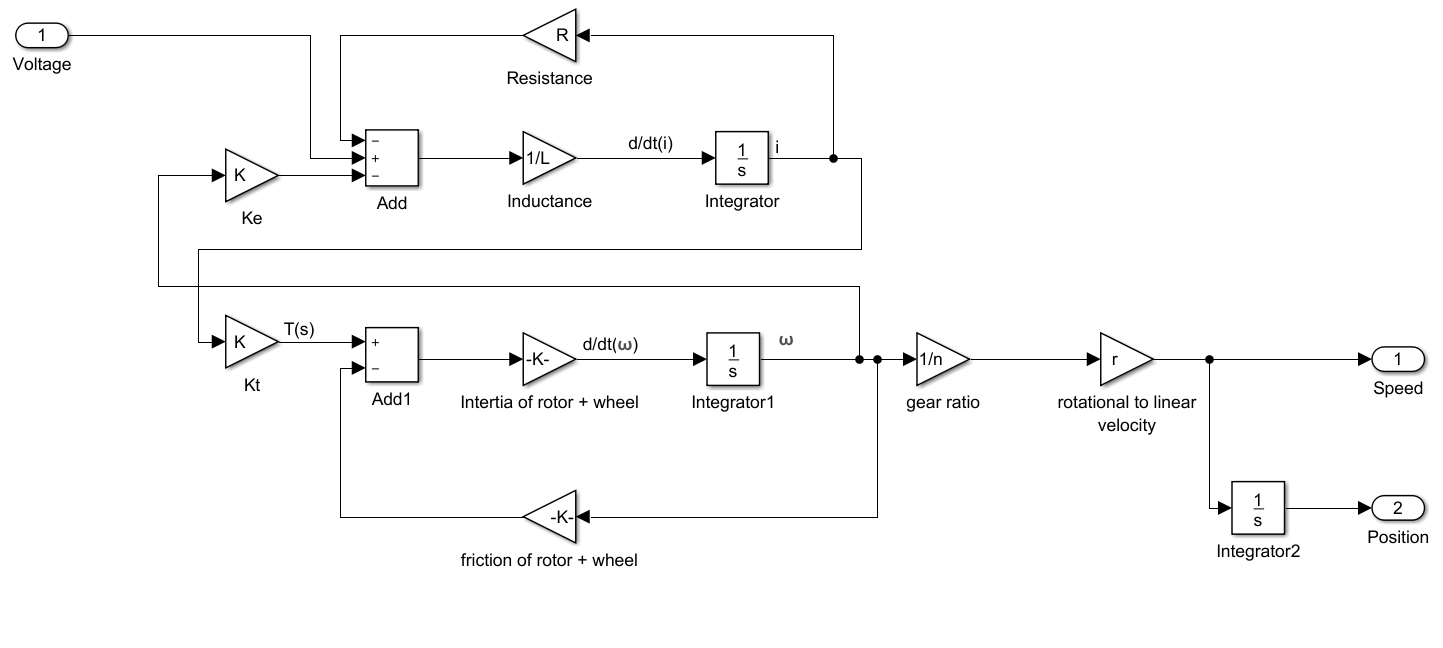
\includegraphics[width=1.1\textwidth]{dc_motorD}
\caption{DC Motor Block Diagram}
\label{fig::dcmfigure}
\end{figure}

The inclusion of the gear ratio (\textbf{n}) and the radius of the wheel (\textbf{r}) products to the angular velocity in the end of the block diagram, results in model scaling for the linear velocity (\textbf{v}) of the wheel. (\ref{eq12})

\begin{equation} \label{eq12}
v = r\omega
\end{equation}

Performing integration on the derived linear velocity results in obtaining the linear displacement of the wheels, later to be used with the kinematics model. 

To summarise, the goal was to relate the voltage to the speed. The input of the block diagram is the voltage of the motor (\textbf{V}) while the outputs are the linear speed caused by wheel rotation and the linear displacement, obtained from integrating the speed. The blocks comprising the upper and lower part of the block diagram, directly correspond to equation \ref{eq11} (upper part correspond to the electrical part of the motor; lower part correspond to the mechanical part of the motor).

Furthermore, as this paper is concerned with the development of a differential drive robot, the block diagram in figure \ref{fig::dcmfigure} is solely a subsystem of the complete kinematics model. That is, two DC motor subsystems are required in order to describe the complete motor/wheel dynamics. 

\section{Kinematics Model of Differential Drive}

Differential drive is a common mechanism in mobile robotics. It consists of two wheels on a common axis, driven by two motor, where each wheel can be independently driven in either forward or backward direction. That is, by varying the velocities of each wheel, different  trajectories could be achieved. Importantly, the rotation the robot performs is based on a point common to the right and left wheel axis, denoted as Instantaneous Center of Curvature(\textbf{ICC}). The kinematic representation can be observed in figure \ref{fig::diff_drive_over} .

\begin{figure}[h]
\centering
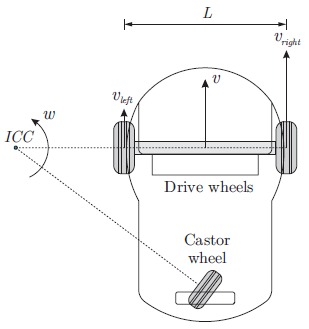
\includegraphics[width = 0.5\textwidth]{Kinematics_char}
\caption{Differential drive overview}
\label{fig::diff_drive_over}
\end{figure}

The linear speed, previously derived from chapter \ref{dc_model}, is represented as $v_r$ and $v_l$, for each of the wheels. The speed of the robot is taken as the average speed of each wheel.

\begin{equation} \label{eq13}
v = \frac{v_r + v_l}{2} 
\end{equation}

The angular speed of the robot (or turning speed) is based on the linear speeds of each wheel and the distance between the wheels. It is denoted as \textbf{W} in equation \ref{eq14}.(not to be confused with $\omega$, the rotational speed of the motor)

\begin{equation} \label{eq14}
W = \frac{v_r - v_l}{l}
\end{equation}

The relation between the linear speed and the angular speed of the robot is similar to equation \ref{eq12}.

\begin{equation} \label{eq15} 
v = WD
\end{equation}

Where D is the turning radius, from the midpoint of the wheels to the ICC. Solving for the turning radius, yields:

\begin{align}
D = \frac{v}{W} \label{eq16} \\
= \frac{l}{2}\frac{v_r + v_l}{v_r - v_l} \nonumber
\end{align}

Analysis of the above equation leads to the consideration of three cases where certain behaviour is to be expected.

\begin{itemize}

\item $\boldsymbol{v_r = v_l}$ \\ In this case scenario, both wheels have the same speed. The robot's speed from equation \ref{eq13} is simply equal to the individual speed of each of wheel. On the other hand, the angular speed from equation \ref{eq14} becomes 0, and the turning radius infinite. The robot is expected to perform straight linear motion.

\item $\boldsymbol{v_r = 0}$ or $\boldsymbol{v_l = 0}$ \\ In this case scenario, the turning radius becomes $\frac{l}{2}$. The robot is expected to perform rotation either about the right or the left wheel, with the center of rotation being the zero velocity wheel. 

\item $\boldsymbol{v_l = -v_r}$ \\ In this case scenario, the turning radius and the linear speed become 0, while the angular speed is doubled. The robot is expected to perform rotation about it's midpoint, or simply put in-place rotation.

\end{itemize}

It is important to mention that the wheels , present in the system , carry some \textbf{nonholonomic} constraints. That is, the robot's local movements are restricted, while no restrictions are present in the global navigation. We can further extend the idea with the use of generalised coordinates.

\begin{equation} \label{eq17}
q = (x,y,\theta) 
\end{equation}

Equation \ref{eq17} could be seen as a point on a two dimensional Cartesian coordinate system, where x and y are the axis and $\theta$ is the angle between the x axis and the point. 

Figure \ref{fig::orientation} shows the robot representation based on the generalised coordinates.

\begin{figure}[h]
\centering
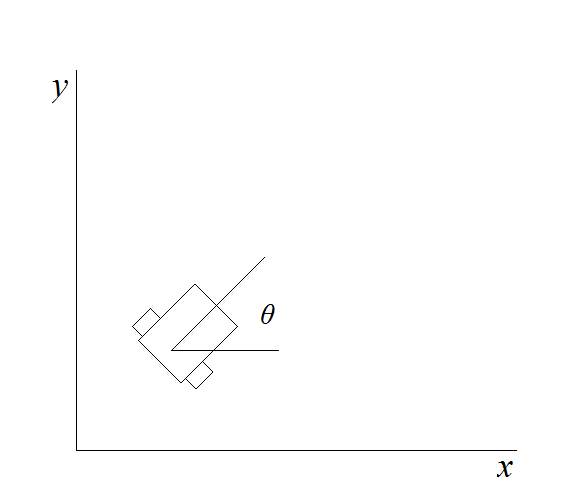
\includegraphics[width = 0.4\textwidth]{Orientation_xy}
\caption{Robot representation in Cartesian coordinates}
\label{fig::orientation}
\end{figure}

We can picture the constrains for the wheels by setting the sideways velocity to zero. That is, the robot can not perform sideways movements like slipping or sliding, but is not limited from manoeuvring in that position, whatsoever. 

\begin{equation} \label{eq18}
\dot{x}sin(\theta) - \dot{y}cos(\theta) = 0
\end{equation}

Equation \ref{eq18} is a common nonholonomic constraint in mobile robotics. \todo{reference to the caltech report}

Particularly if the robot is viewed as a point, the Kinematics equations in Cartesian space can be derived as:

\begin{align}
\dot{x} = vcos(\theta) \nonumber \\
\dot{y} = vsin(\theta) \label{eq19} \\
\dot{\theta} = \omega  \nonumber 
\end{align}

In the case of a differential drive robot, substitution of the linear and angular velocities, \textbf{v} and $\boldsymbol{\omega}$, with the previously derived in equation \ref{eq13} and \ref{eq14} average robot speed and angular robot speed (with respect to the center of rotation between the wheels), will results in the kinematics equations for locomotion of a differential drive. 

\begin{align}
\dot{x} = \frac{v_r + v_l}{2}cos(\theta) \nonumber \\
\dot{y} = \frac{v_r + v_l}{2}sin(\theta) \label{eq20} \\
\dot{\theta} = \frac{v_r - v_l}{l} \nonumber
\end{align}

In equation \ref{eq20} we will have a change in the robot's position (x,y,$\theta$) when the velocity of each wheel is controlled. 

\subsection{Kinematics in simulink} 

\begin{table}[h]
\centering
\begin{tabular}{cccll}
\hline
Parameter                   & Description                               &  &  \\ \hline
\multicolumn{1}{|c|}{l}     & \multicolumn{1}{c|}{Distance between wheels}       &  &  \\ \cline{1-2}
\multicolumn{1}{|c|}{$v_r$} & \multicolumn{1}{c|}{Linear speed of right wheel}  &  &  \\ \cline{1-2}
\multicolumn{1}{|c|}{$v_l$} & \multicolumn{1}{c|}{Linear speed of left wheel}  &  &  \\ \cline{1-2}
\multicolumn{1}{|c|}{v}     & \multicolumn{1}{c|}{Average linear robot speed}  &  &  \\ \cline{1-2}
\multicolumn{1}{|c|}{W}     & \multicolumn{1}{c|}{Angular robot speed}        &  &  \\ \cline{1-2}
\multicolumn{1}{|c|}{D}     & \multicolumn{1}{c|}{Turning radius}         &  &  \\ \cline{1-2}
\multicolumn{1}{l}{}        & \multicolumn{1}{l}{}                      &  &  \\ \hline
\end{tabular}
\caption{Kinematics parameters}
\label{kin_para}
\end{table}

Using equations \ref{eq13} and \ref{eq14} a simulink block diagram is constructed in figure \ref{fig::diff_simulink}.

\begin{figure}[h]
\centering
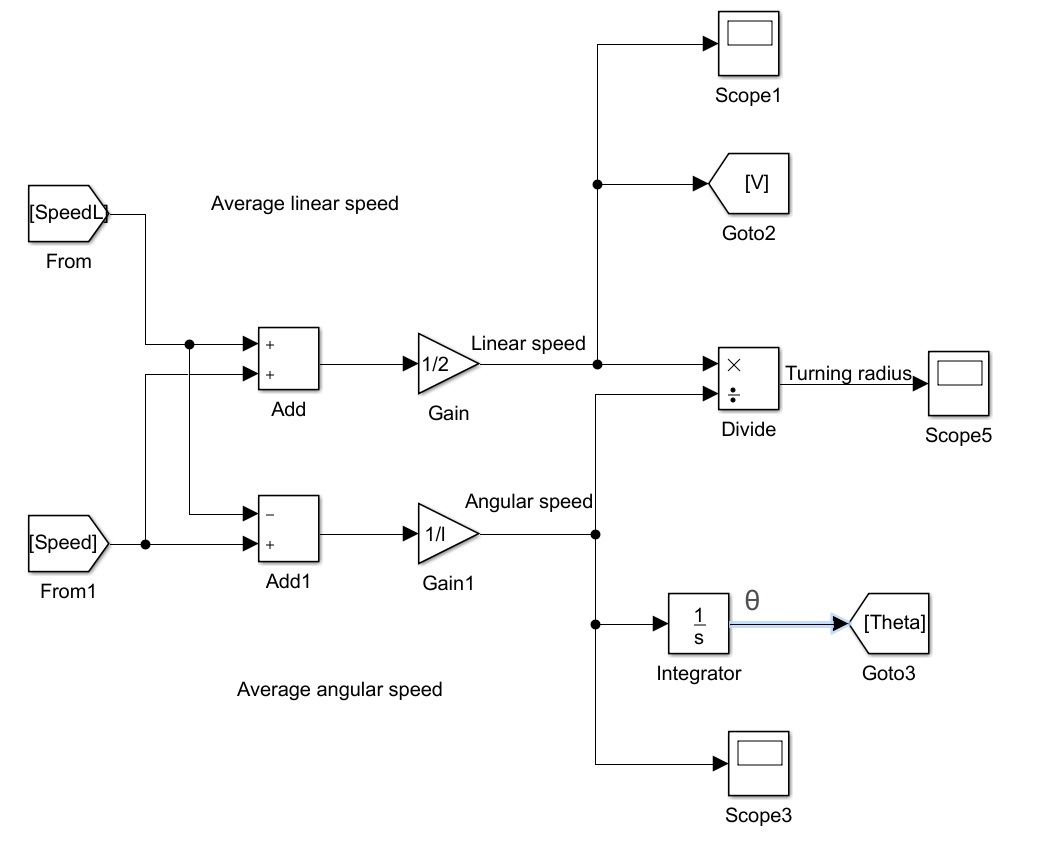
\includegraphics[width = 0.8\textwidth]{diff_drive_kin_simulink}
\caption{Differential drive kinematics}
\label{fig::diff_simulink}
\end{figure} 

The inputs are the individual wheel velocities, arranged to reflect the previously mentioned equations. The middle output is the turning radius \textbf{D}, which is governed by equation \ref{eq16}. The derived average linear speed is to be further used in equation \ref{eq20} to estimate the position of the robot based on it's angle through time, where the angle ($\theta$) is   obtain from integrating $\dot{\theta}$, which itself is the angular speed of the robot. 

\begin{figure}[h]
\centering
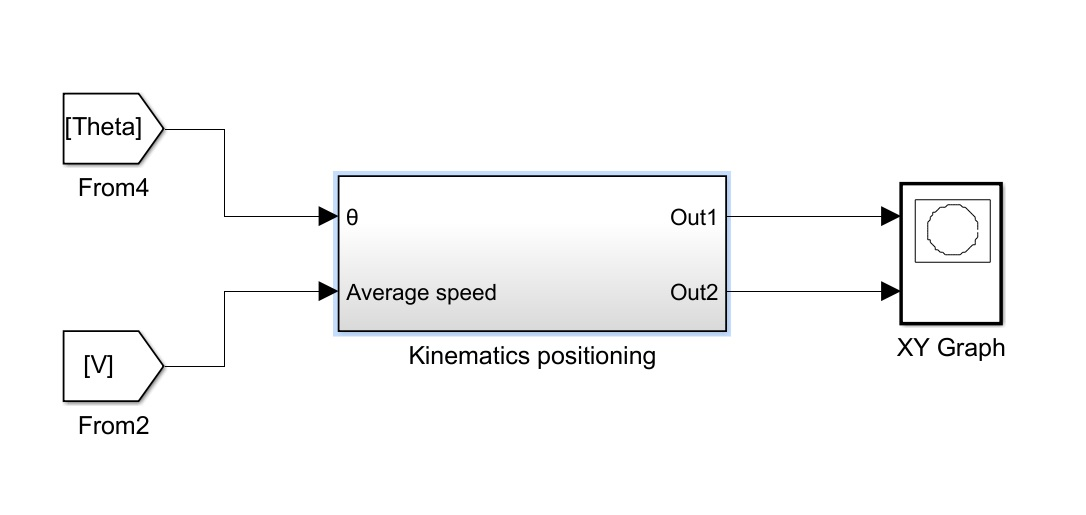
\includegraphics[width = 0.8\textwidth]{kin_pos_subsystem}
\caption{Positioning subsystem}
\label{fig::pos_sub}
\end{figure} 

In figure \ref{fig::pos_sub} the inputs are the the average speed and the orientation of the robot, while the outputs X and Y from equation \ref{eq20} are fed in a graph to observe the robot's trajectory through time. 

\begin{figure}[h]
\centering
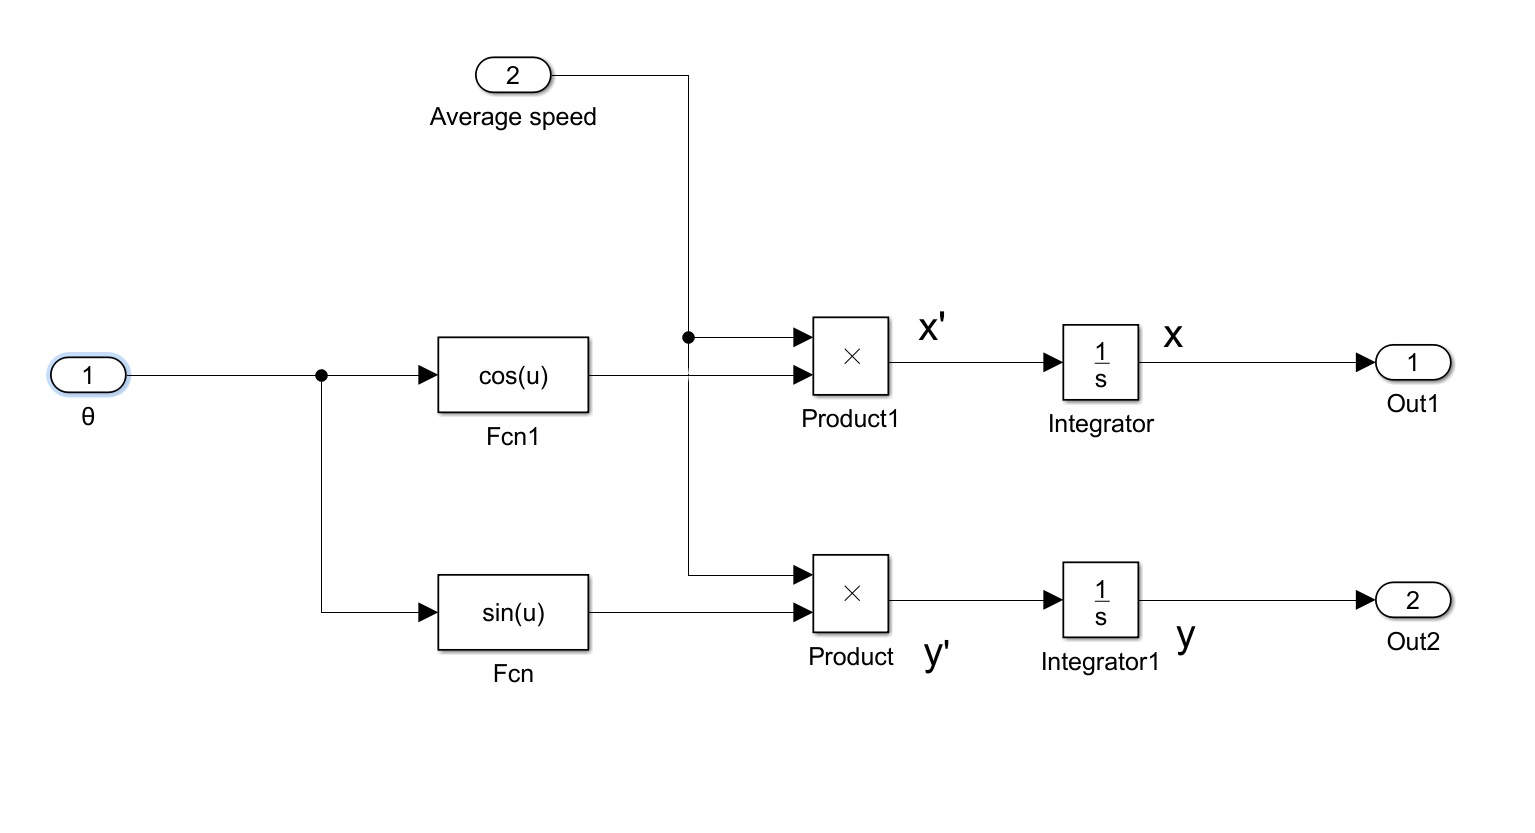
\includegraphics[width = 0.8\textwidth]{kin_model_pos}
\caption{Positioning subsystem}
\label{fig::pos_model}
\end{figure} 

The subsystem from figure \ref{fig::pos_sub} is composed of blocks arranged to reflect equation \ref{eq20}. The outputs $\dot{x}$ and $\dot{y}$ are further integrated to graph the trajectory of the robot. 

\section{Complete model}
\chapter{Hardware}\label{ch:hardware}

\paragraph{Hardware in the device} 



In the following chapter we will see what hardware we have used to produce this device.
First we decided on what platform we will be working on.

\section{Single board computer} 

Since we were allready familiar with the Raspberry Pi singleboard computer we decided that it is best to continue with the system we are allready know how to operate.
At first we used the Raspberry Pi 2 model B but in concideration of the power supply and performance we swapped it out with a Raspberry Zero.


\begin{figure}[h]
\centering
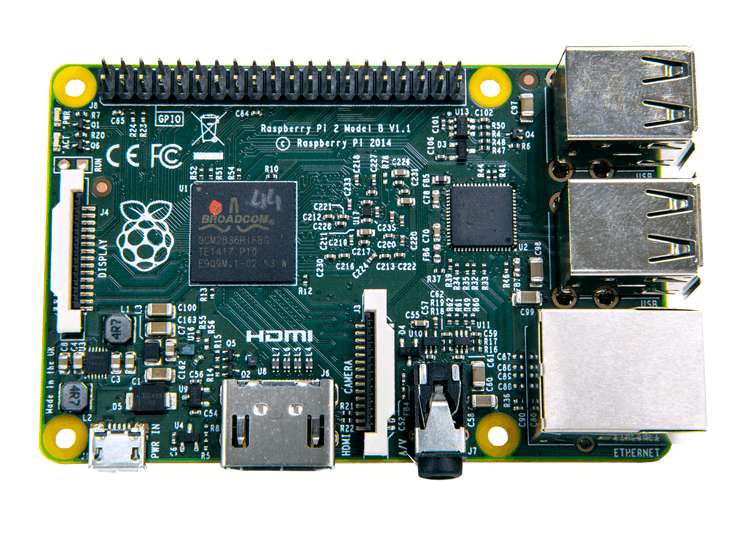
\includegraphics[width = 0.5\textwidth]{Raspberry-Pi-2}
\caption{Raspberry Pi 2B}
\label{fig::rasppi2b}
\end{figure}

\begin{figure}[h]
\centering
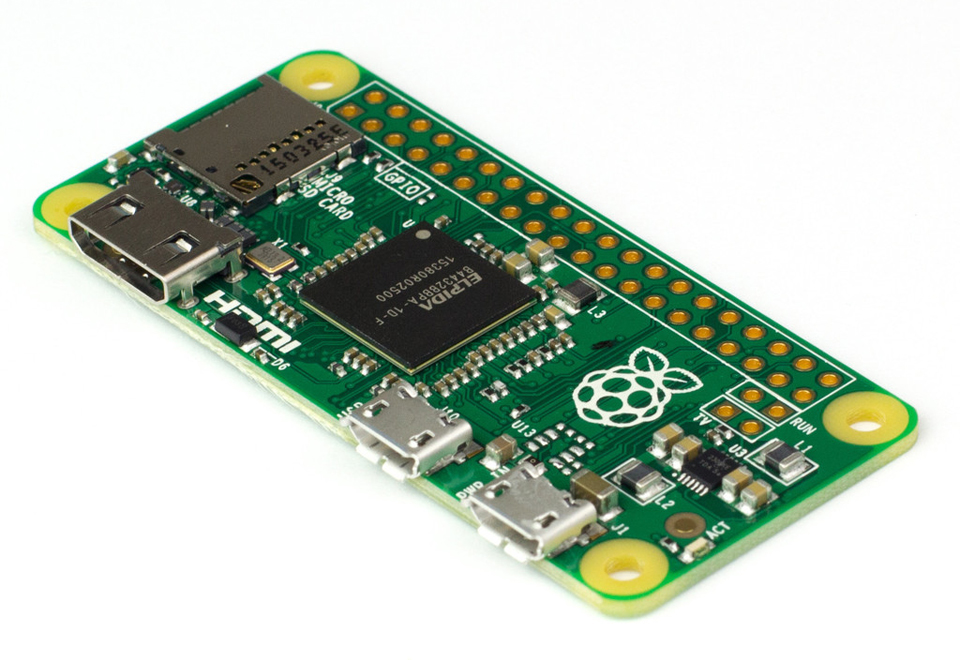
\includegraphics[width = 0.5\textwidth]{raspberry_pi_zero_1}
\caption{Raspberry Pi Zero}
\label{fig::raspizero}
\end{figure}


We chose the Rasperry Pi Zero over the Raspberry Pi 2B because of the lesser power consumption and the size.
Performance of the two computers are similar. 
Zero has less RAM but in our project it does not have a significant impact.

Specs of the Raspberry Pi Zero:
1Ghz, Single-core CPU
512MB RAM
Mini HDMI and USB On-The-Go ports
Micro USB power
HAT-compatible 40-pin header
Composite video and reset headers



\section{Distance measuring} 

Since our device would be avoiding obstacles on the way it is fitted with distance measuring sensors.
We have decided to use ultra sonic sensors.
Concidering the cost and the performance we are looking for we eventually settled on the HC-SR04 ultra sonic sensor.
In our device we have used three of those sensors in orded to cover the front side of the veichle.

\begin{figure}[h]
\centering
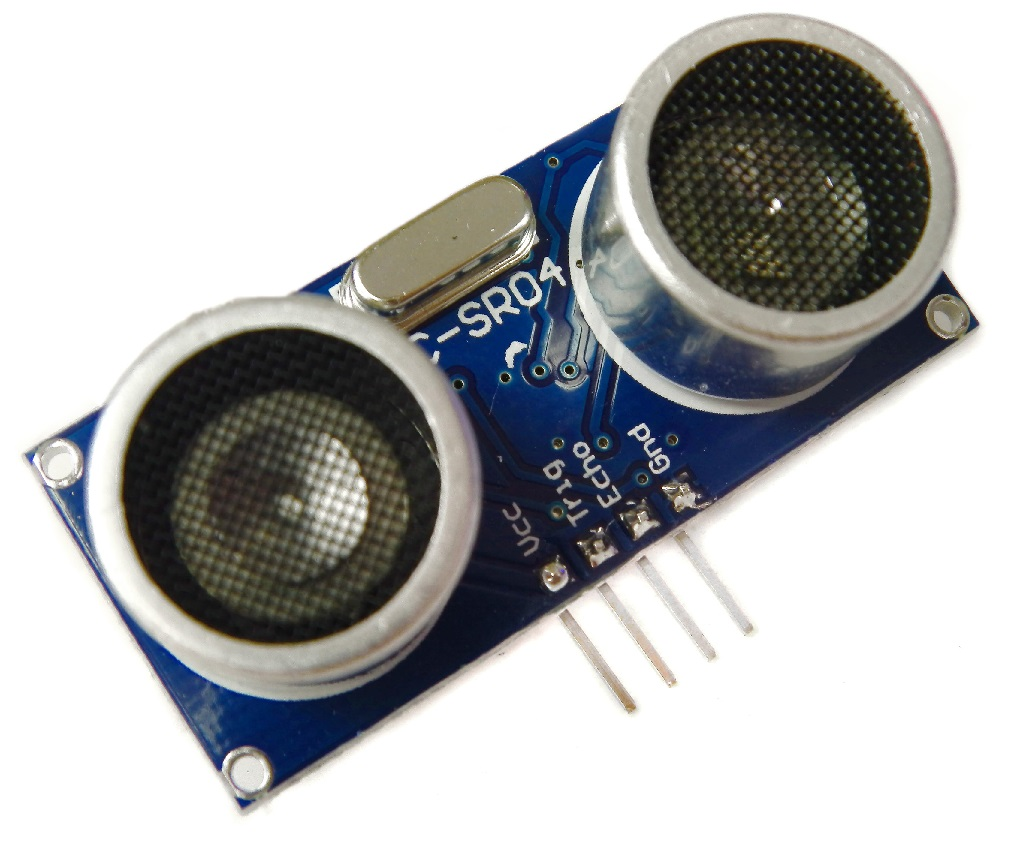
\includegraphics[width = 0.5\textwidth]{hc-sr04}
\caption{Ultra sonic sensor HC-SR04}
\label{fig::hcsr04}
\end{figure}

\section{DC motors and the chassie} 

We are using a premade complect of two DC motors and the chassie with the wheels.
Each of the motors are connected to the wheels directly.

\begin{figure}[h]
\centering
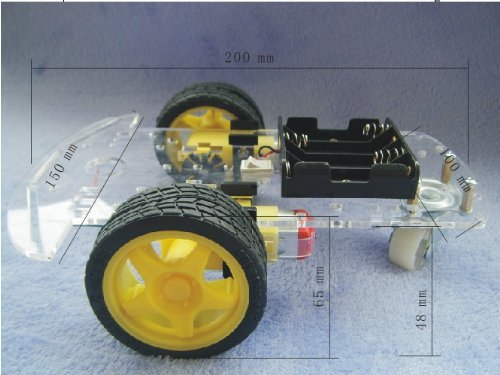
\includegraphics[width = 0.5\textwidth]{chassie}
\caption{Chassie and the two DC motors with a power supply}
\label{fig::chassie}
\end{figure}

Motor specs:

 Voltage:
DC 3V
DC 5V
DC 6V
Current:
100 MA
100MA
120MA
Reduction rate:48:1
RPM (With tire):100,190,240
Tire Diameter:66mm
Car Speed(M/minute):20,39,48

Motor Weight (g):50

Motor Size:70mm*22mm*18mm

Noise:<65dB 

The two motors are identical and are used to move the device and to steer aswell

\section{Motor driver} 

At the beginning of the project we used a L9110S DC Stepper Motor Driver H-Bridge for controlling the movement of the wheels, but as we soon dicovered the suggested driver was not capable of regulating the motor speeds.
To controll the speed of the veichle we then swapped it to the L298N driver.
The second driver was capable of using the PWM to regulate the speed of the motors.

\begin{figure}[h]
\centering
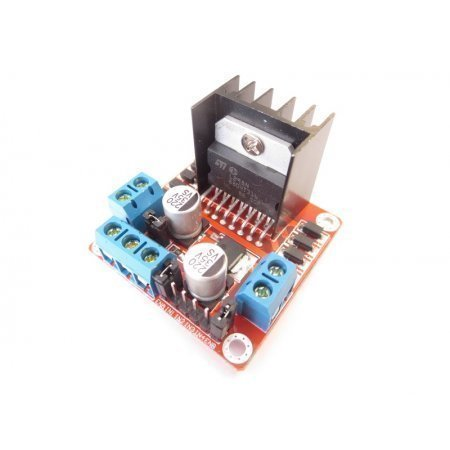
\includegraphics[width = 0.5\textwidth]{driver2}
\caption{The L298N driver}
\label{fig::driver2}
\end{figure}

Driver specs:
Working mode:	H bridge (double lines)
Control chip:	L298N (ST)
Logical voltage:	5V
Driving voltage:	5V-35V
Logical current:	max 36mA
Driving current:	2A (max single bridge)
Maximum power:	25W
Storage temperature:	-20 °C +135 °C
Periphery dimension:	43 x 43 x 27mm(L x W x H)

\section{Speed sensor}

The speed of the wheels is measured by the LM393 IR speed sensors.

\begin{figure}[h]
\centering
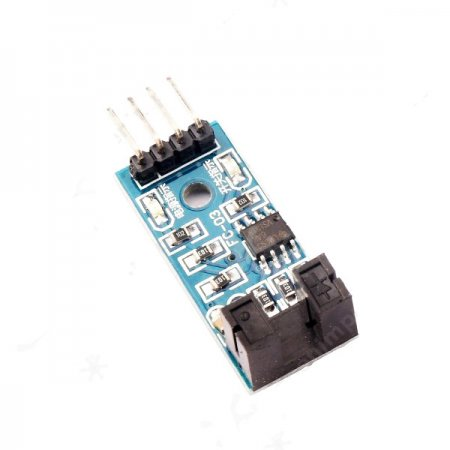
\includegraphics[width = 0.5\textwidth]{irspeed}
\caption{The LM393 IR speed sensor}
\label{fig::driver2}
\end{figure}

The speed sensor is used to estimate the error of the wheel speed.
Features:

Working voltage: 3.3V~5V
Weight: 8g
Dimensions: Approx.3.2 x 1.4 x 0.7cm
5mm Groove width
Using wide voltage LM393 comparator
Application: Widely used in dynamo speed detecting, pulse counting, etc
Output form: Digital switch output (0 and 1) and Analog for Sensitivity.
(CITE:http://www.banggood.com/LM393-Speed-Sensor-Detection-Speed-Module-For-Arduino-p-970033.html?currency=AUD&utm_source=myshopping&utm_medium=cpc&utm_content=saul&utm_campaign=xie-AU)

\section{Wi-Fi dongle}

For the monitoring of the device and connectivity we have used a Edimax EW-7811Un Wi-Fi adapter.

\begin{figure}[h]
\centering
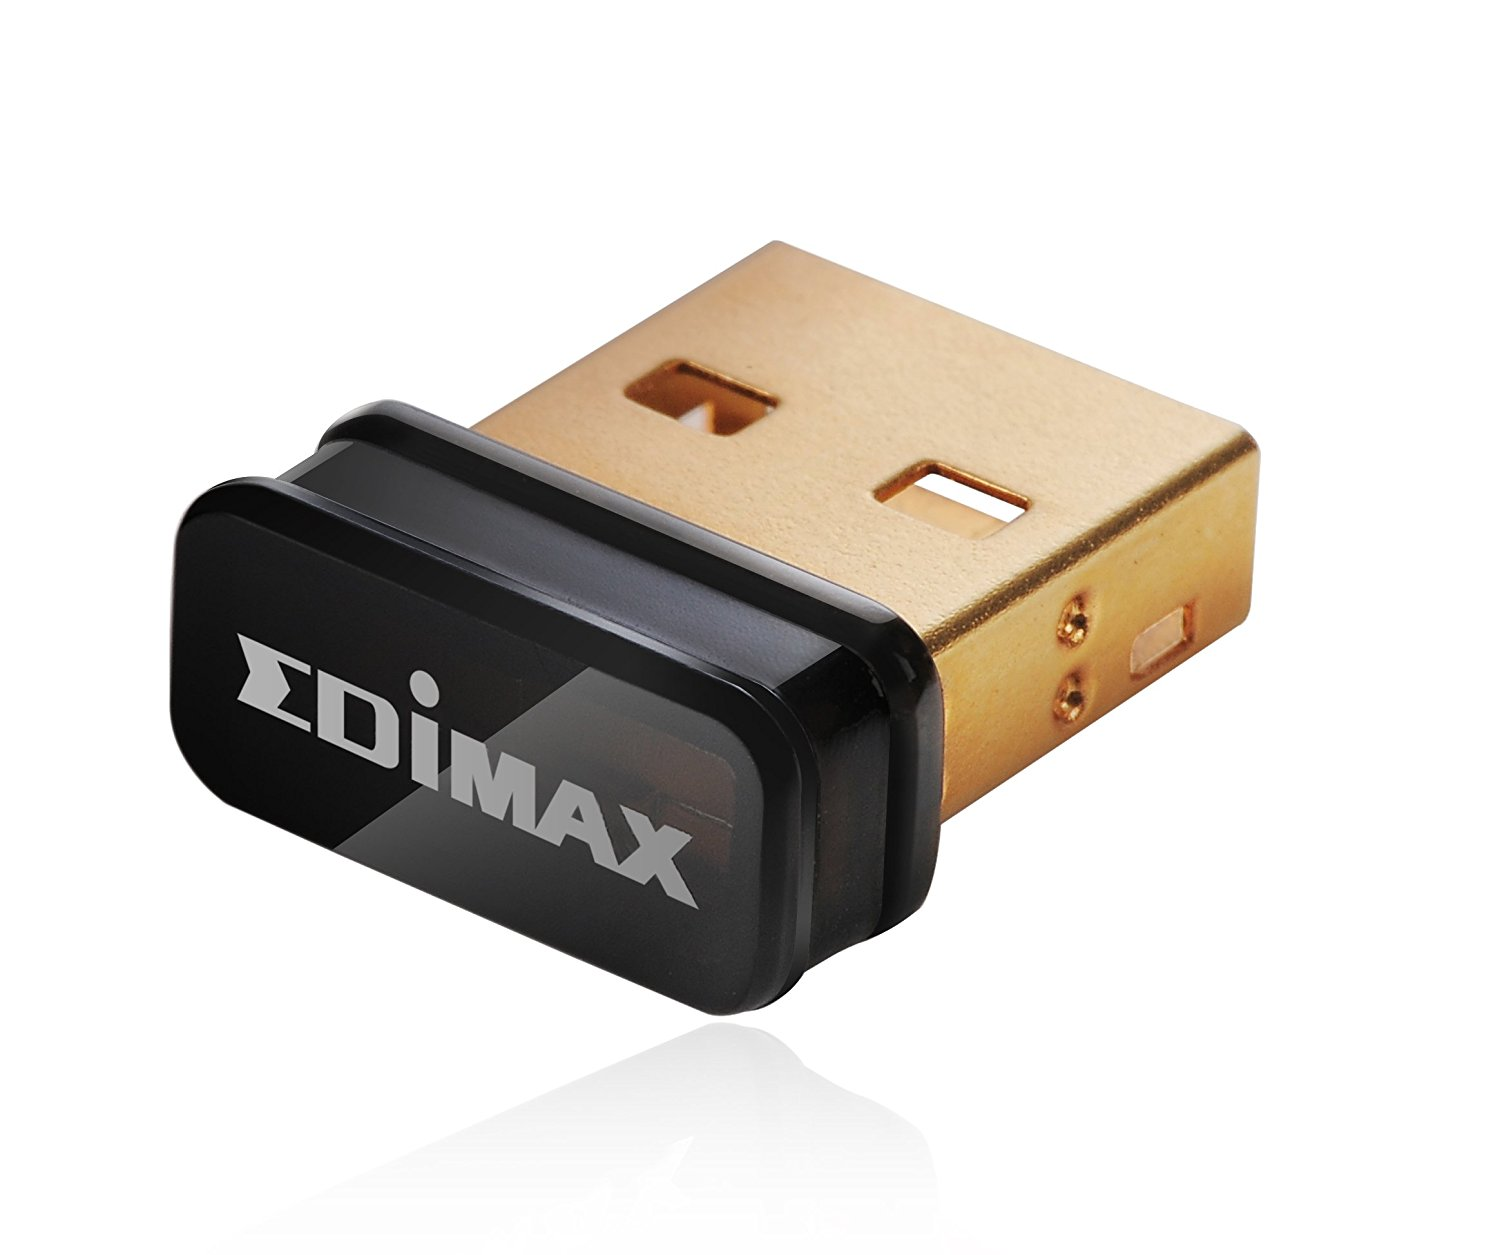
\includegraphics[width = 0.5\textwidth]{edimax}
\caption{Edimax EW-7811Un Wi-Fi adapter}
\label{fig::edimax}
\end{figure}

\section{Assambly}

In this section we will be looking more closely what has been connected to what and how.
From the figure below we can see the layout of the whole system.

\begin{figure}[h]
\centering
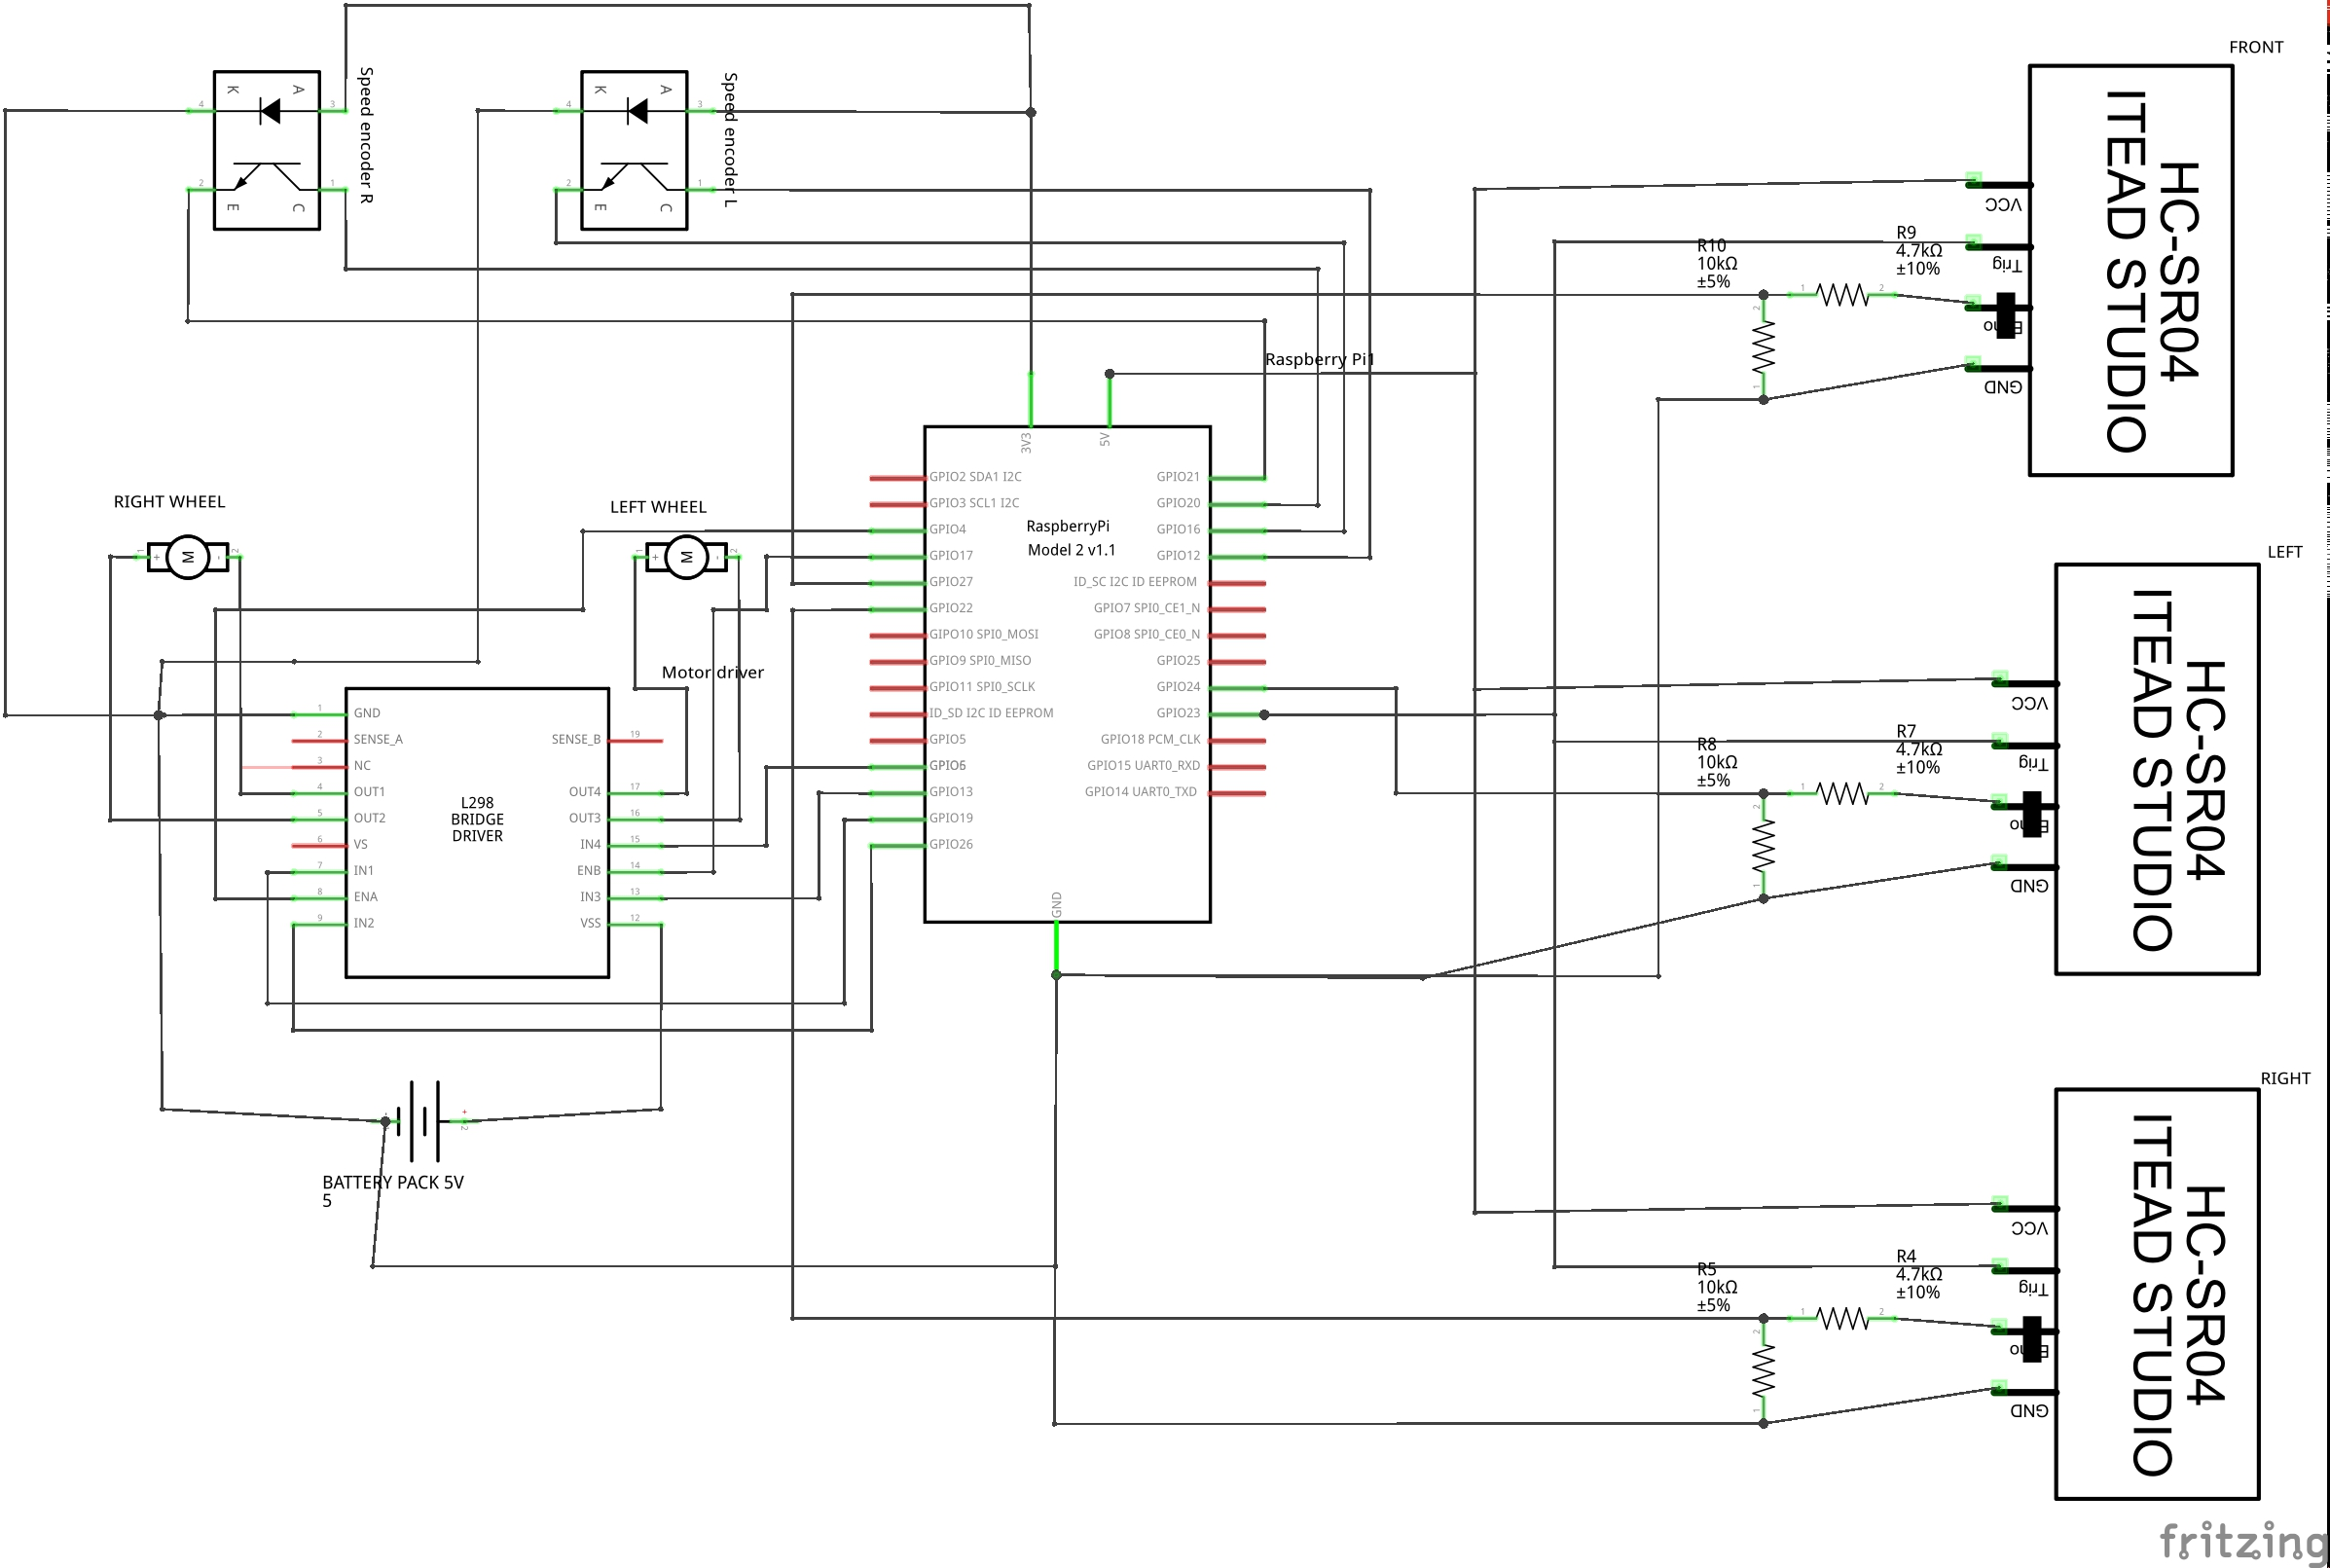
\includegraphics[width = 0.5\textwidth]{P51_schem}
\caption{Schematics of the device}
\label{fig::schematics}
\end{figure}

In the middele you can see the Raspberry Pi.
Since the software used to make this schematic did not have the Raspberry Pi Zero layout we used model 2 instead.
Regarding our project id does not make a difference, since the pins are the same as Zero.

On the right side of the system you can see three ultrasonic sensors.
The ultrasonic sensors are connected to the RP Pi.
The Vcc and GND pins all go to the Raspberry so that the power for the sensors is taken from the Raspberry itself.
The triger pins all go to the same Raspberry pin.
That means that when you trigger one of the sensors all of them will emit sonic impulse.
The trigers are all on the same pin to preserv more pins on the Raspberry, it does not matter if they are on one or seperate pins.
The echo pins of each of the sensors go into seperate ports on the Raspberry, each of them has a voltage divider connected to the GND as well.

In the left bottom you can see the driver with the motors and a seperate battery pack.
The battery pack is connected to the driver to give power to the motors and the driver itself aswell.
Driver is connected to the Raspberry by 6 pins.
Four of the pins are for the directions of the both motors.
Two of the pins what are the enable pins are used for controlling the speed of the motors by PWM.
The motors are connecter directly to the driver by two wires.
In the top left you can see the two encoders what are used for monitoring the speed of the wheels.

For the Raspberry we have a external power source what is not pictured on the figure.


\chapter{Development}\label{ch:development}

\paragraph{Hardware testing} 

\section{Ultrasonic sensors}

First of the hardware we started testing the ultrasonic sensors.
For each of the sensors we built a voltage divider seen on the following figure.

\begin{figure}[h]
\centering
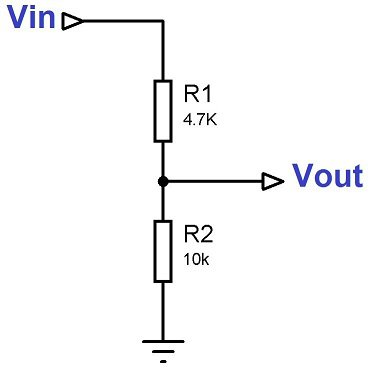
\includegraphics[width = 0.5\textwidth]{voltage1}
\caption{Voltage divider}
\label{fig::voltage1}
\end{figure}

The values of the resistors are calculated by the following equation:
\begin{equation} \label{voltagedivider} 
{V}_{out}={V}_{in}*{R}_{2}/({R}_{1}+{R}_{2})
\end{equation}

We tried all the sensors out seperately by connecting them 1 by 1 to the raspberry and ran the test code.

\begin{lstlisting}
import RPi.GPIO as GPIO
import time
GPIO.setmode(GPIO.BCM)

TRIG = 23
ECHO = 24

print "Measuring distance"

GPIO.setup(TRIG, GPIO.OUT)
GPIO.setup(ECHO, GPIO.IN)

while True:
	GPIO.output(TRIG, False)
	print "W8ing on da sensor"
	time.sleep(2)

	GPIO.output(TRIG, True)
	time.sleep(0.00001)
	GPIO.output(TRIG, False)

	while GPIO.input(ECHO)==0:
		pulse_start = time.time()

	while GPIO.input(ECHO)==1:
		pulse_end= time.time()

	pulse_duration = pulse_end - pulse_start

	distance = pulse_duration * 17150
	distance = round(distance, 2)

	print "Distance:%d",distance

\end{lstlisting}

Each of the sensors worked correctly while connected seperately so we moved on to try them out all of them at the same time.
For that we connected all of the ultrasonic sensors to the raspberry and tried them out.
For testing all of them we included some filtering aswell, because while taking every reading we saw that some of the values where off the chart high.
High values was most probably due to the noise or just some random jittering.
Our filter is made to take three readings at the time and then calculate the average.

\begin{lstlisting}
def readsensor(PIN):
	for x in range(0, 2):
		read_time_start1 = time.time()
		GPIO.output(TRIG, True)
		time.sleep(pulse)
		GPIO.output(TRIG, False)

		while GPIO.input(PIN)==0:
			pulse_start = time.time()

		while GPIO.input(PIN)==1:
			pulse_end= time.time()

		pulse_duration[x] = pulse_end - pulse_start
		time.sleep(0.05-(time.time()-read_time_start1))

	distance = sum(pulse_duration)/measurment_count* SPEED_OF_SOUND
	distance = round(distance, 2)
	print distance
while True:
	readsensor(ECHOF)
	readsensor(ECHOR)
	readsensor(ECHOL)
	
\end{lstlisting}

As you can see from the code above we made sure that every reading takes exactly 0.05 seconds.
This will help us make every cycle evenly long and we can predict the total time that the program runs the whole cycle.
After applying the filter we saw that the readings became alot more percise and consistent.
Therefore the time for the sensor reading loop becomes 3*0,05s=0,15s.

\section{DC motors}

For testing the dc motors we drove the motors in forward gear and in backward gear through the driver we are useing.
Below you can see the script we used to conduct the testing of the motors.

\begin{lstlisting}
GPIO.setmode(GPIO.BCM)
GPIO.setup(StepPinForward, GPIO.OUT)
GPIO.setup(StepPinBackward, GPIO.OUT)

def forward(x):
    GPIO.output(StepPinForward, GPIO.HIGH)
    print "forwarding running  motor "
    time.sleep(x)
    GPIO.output(StepPinForward, GPIO.LOW)

def reverse(x):
    GPIO.output(StepPinBackward, GPIO.HIGH)
    print "backwarding running motor"
    time.sleep(x)
    GPIO.output(StepPinBackward, GPIO.LOW)

print "forward motor "
forward(5)
print "reverse motor"
reverse(5)

print "Stopping motor"
GPIO.cleanup()

\end{lstlisting}

As you can see from the code it runs one of the two motors first forward for 5 seconds and then backwards for 5 seconds.
For the second motor we just changed the pin numbers(StepPinForward and StepPinBackward).

\chapter{Conclusion}\label{ch:conclusion}
In case you have questions, comments, suggestions or have found a bug, please do not hesitate to contact me. You can find my contact details below.
  \begin{center}
    Jesper Kjær Nielsen\\
    \href{mailto: jkn@es.aau.dk}{jkn@es.aau.dk}\\
    \href{http://kom.aau.dk/~jkn}{http://kom.aau.dk/\textasciitilde jkn}\\
    Fredrik Bajers Vej 7\\
    9220 Aalborg Ø
  \end{center}

\printbibliography[heading=bibintoc]
\label{bib:mybiblio}
\appendix
\chapter{Driver chip}\label{ch:appAlabel}

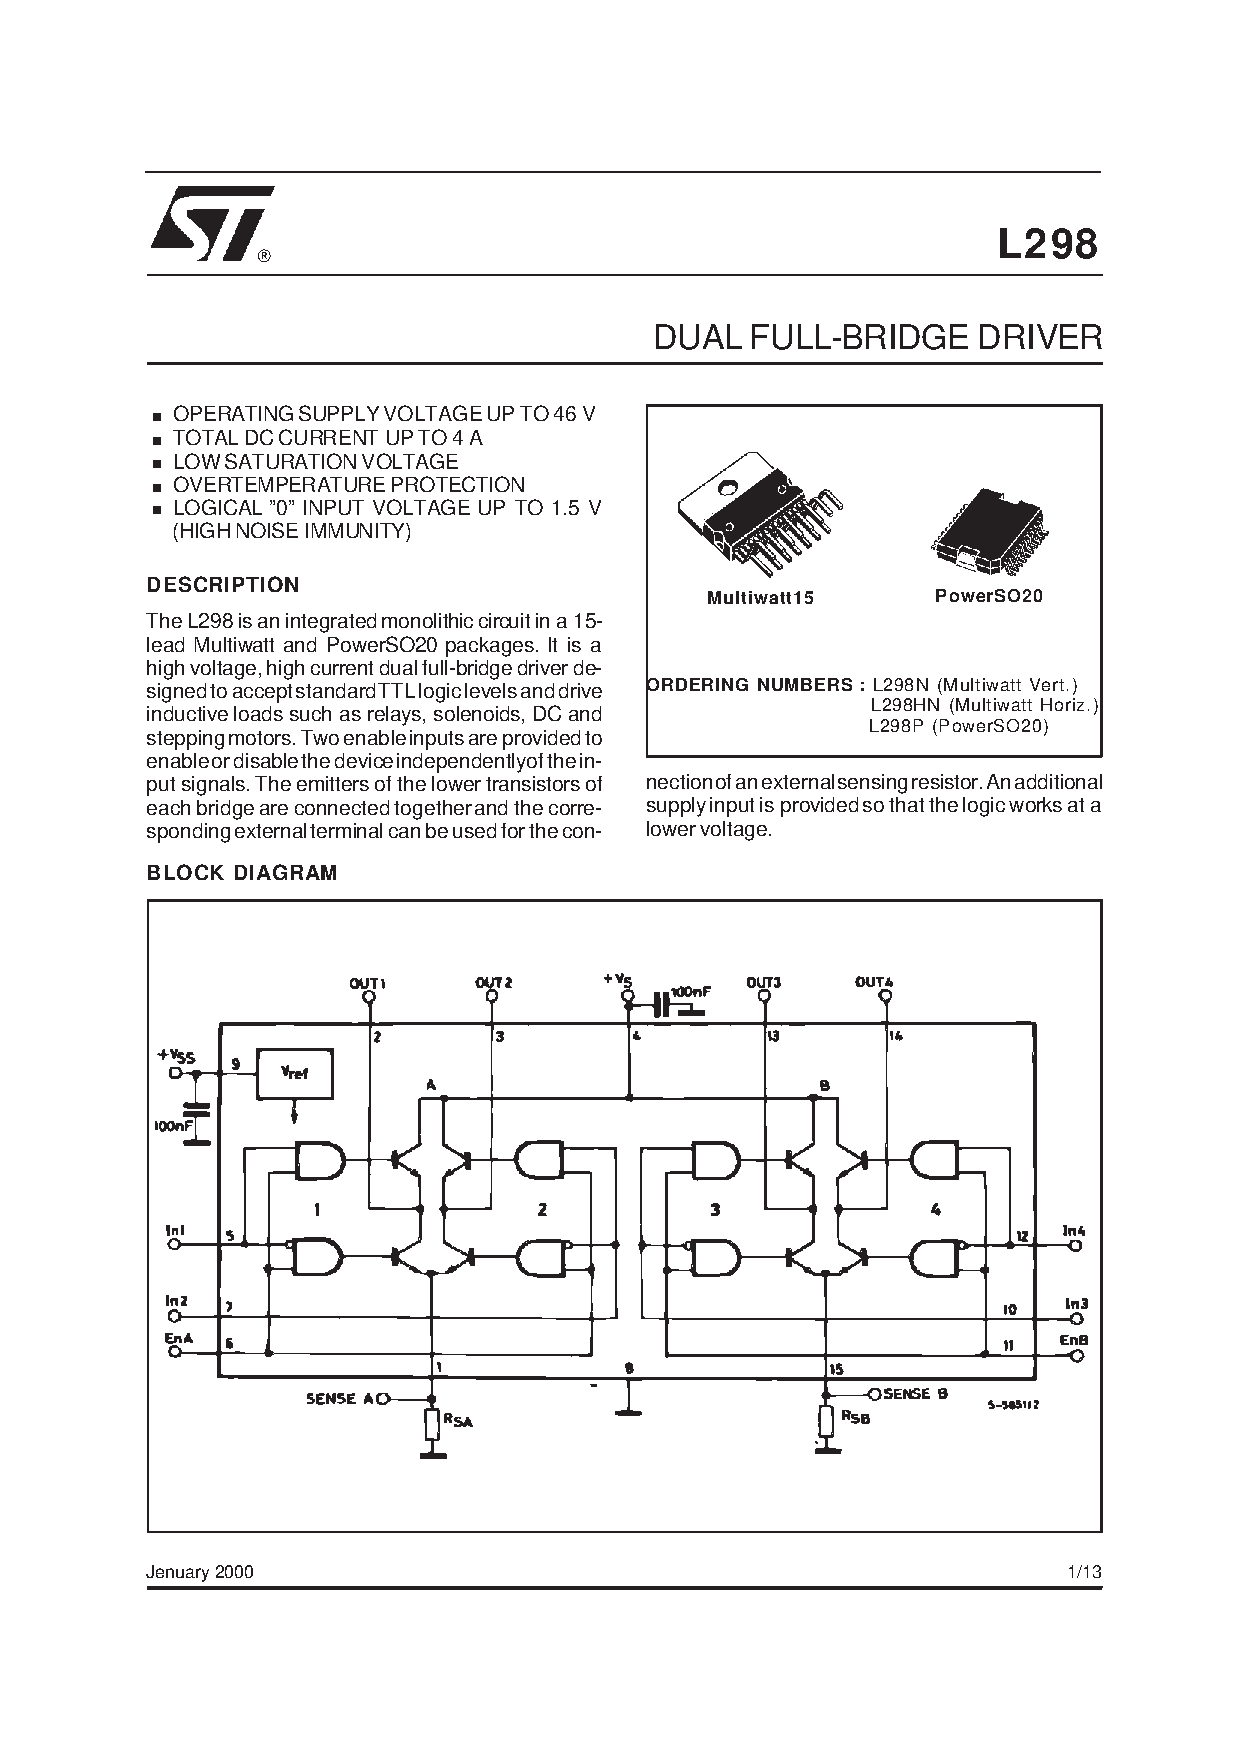
\includepdf[
pages=-,
width=1.6\textwidth,
height=1\textheight,
angle=0,
pagecommand =\section*{Driver Chip}]{datasheets/driverchip.pdf}

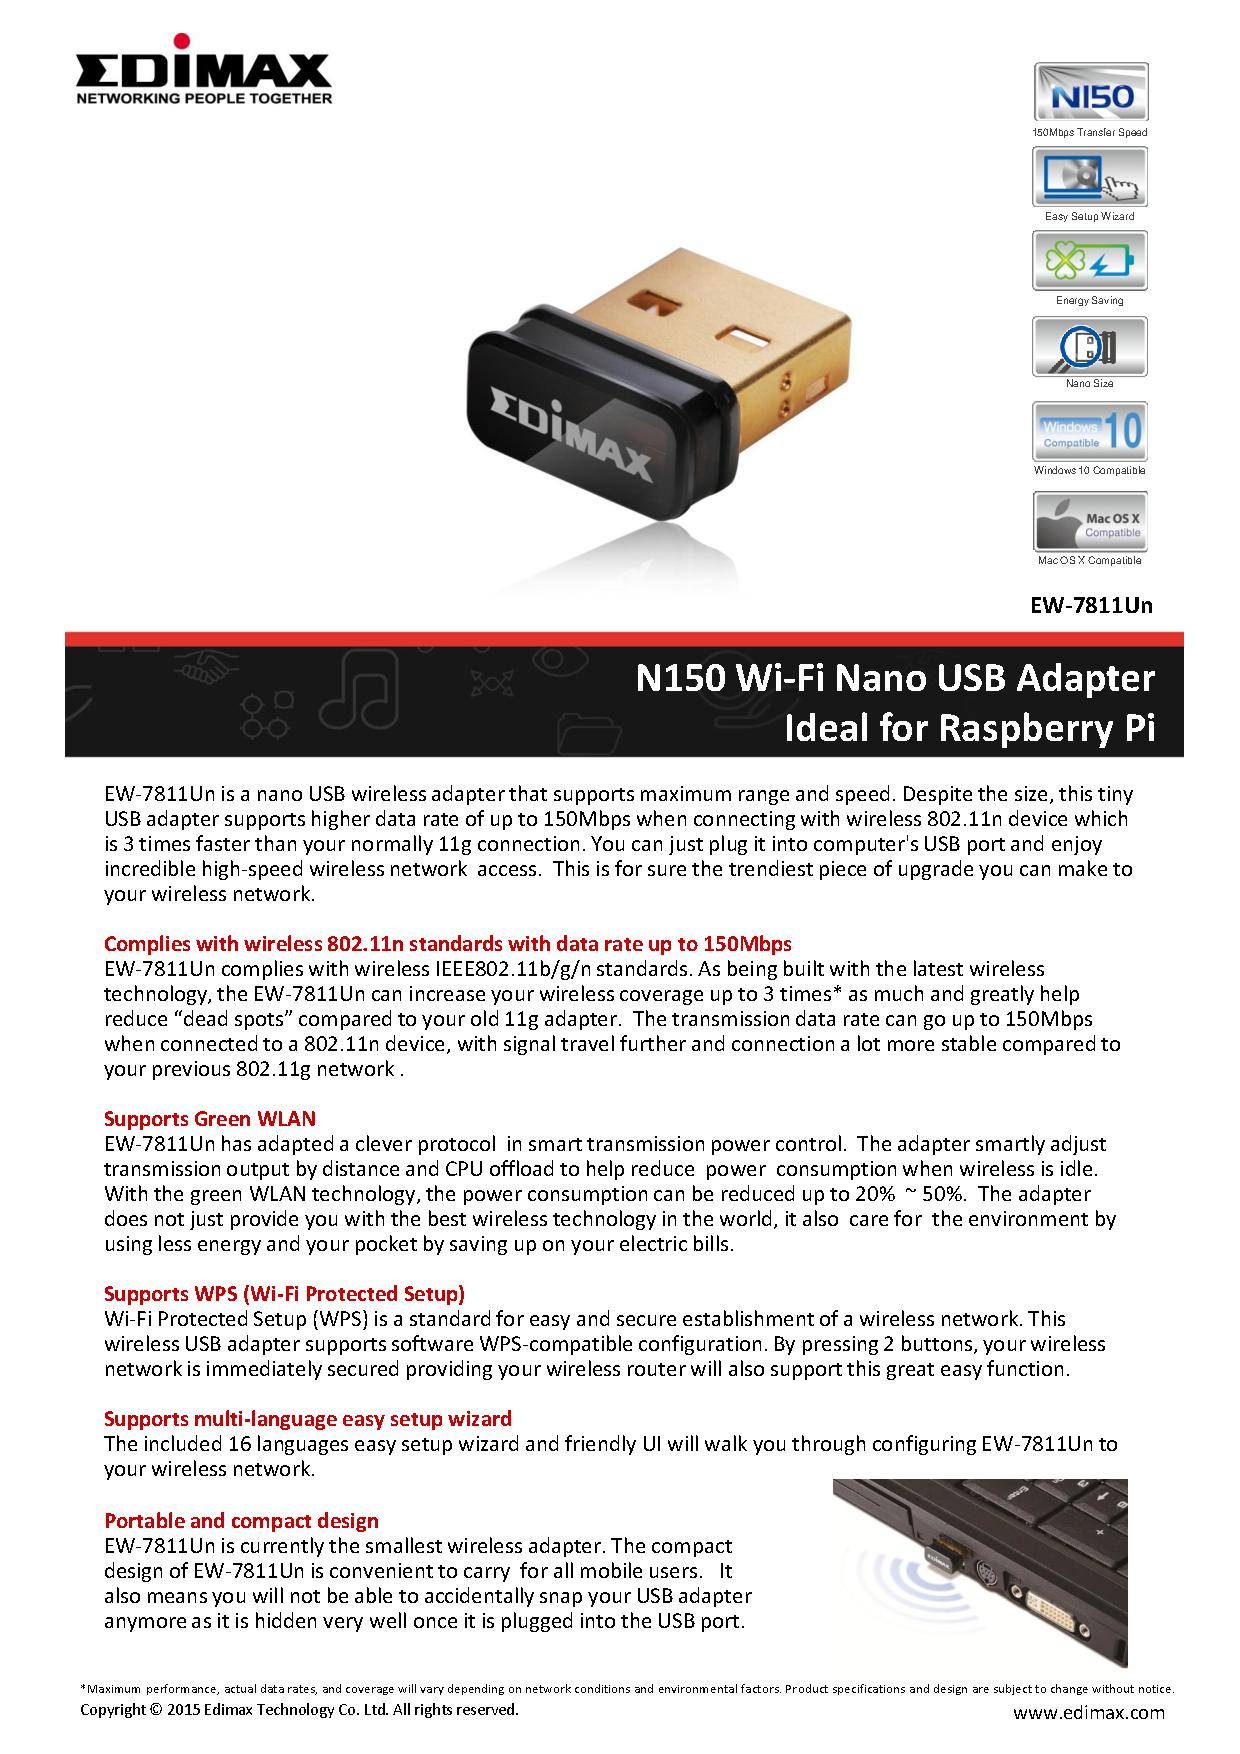
\includepdf[
pages=-,
width=1.6\textwidth,
height=1\textheight,
angle=0,
pagecommand =\section*{Driver Chip}]{datasheets/EW-7811Un_Datasheet_English.pdf}

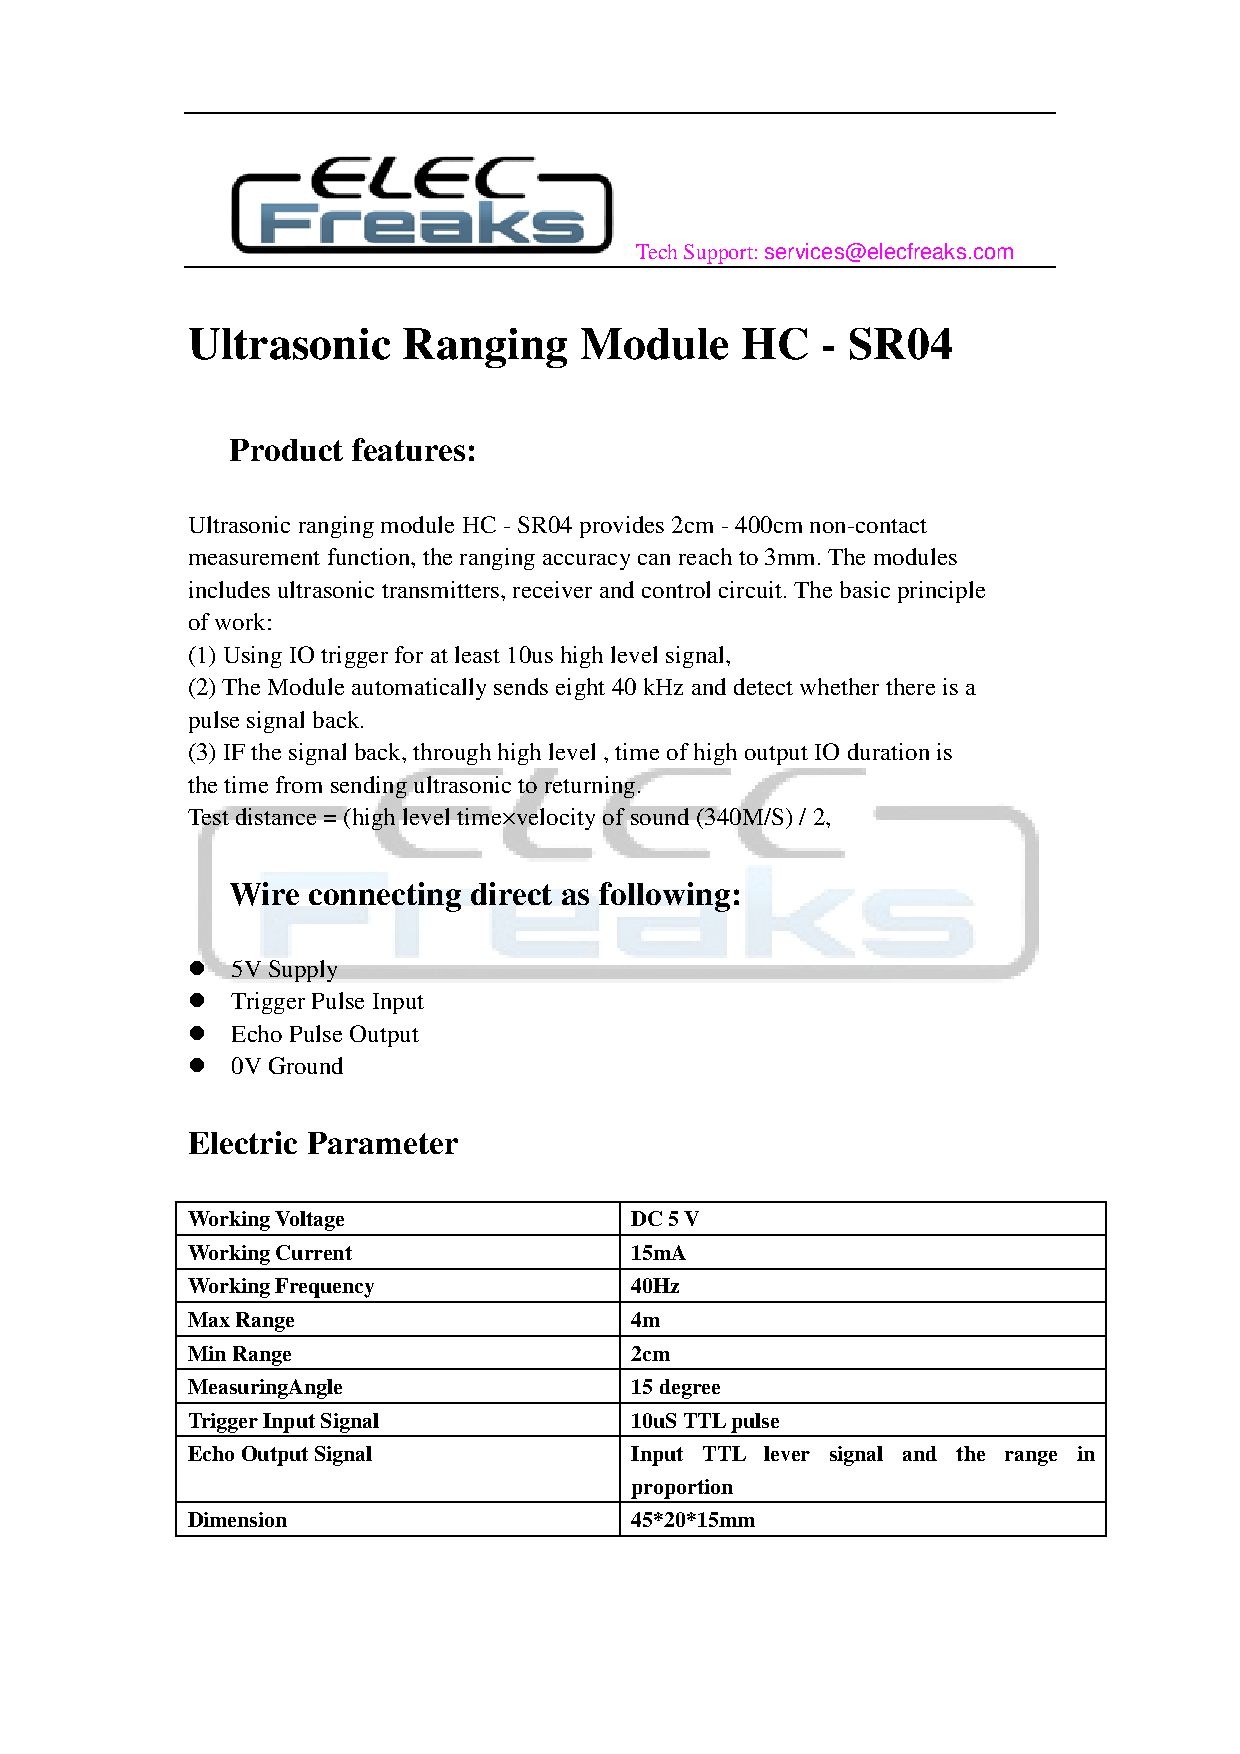
\includepdf[
pages=-,
width=1.6\textwidth,
height=1\textheight,
angle=0,
pagecommand =\section*{Driver Chip}]{datasheets/HCSR04.pdf}

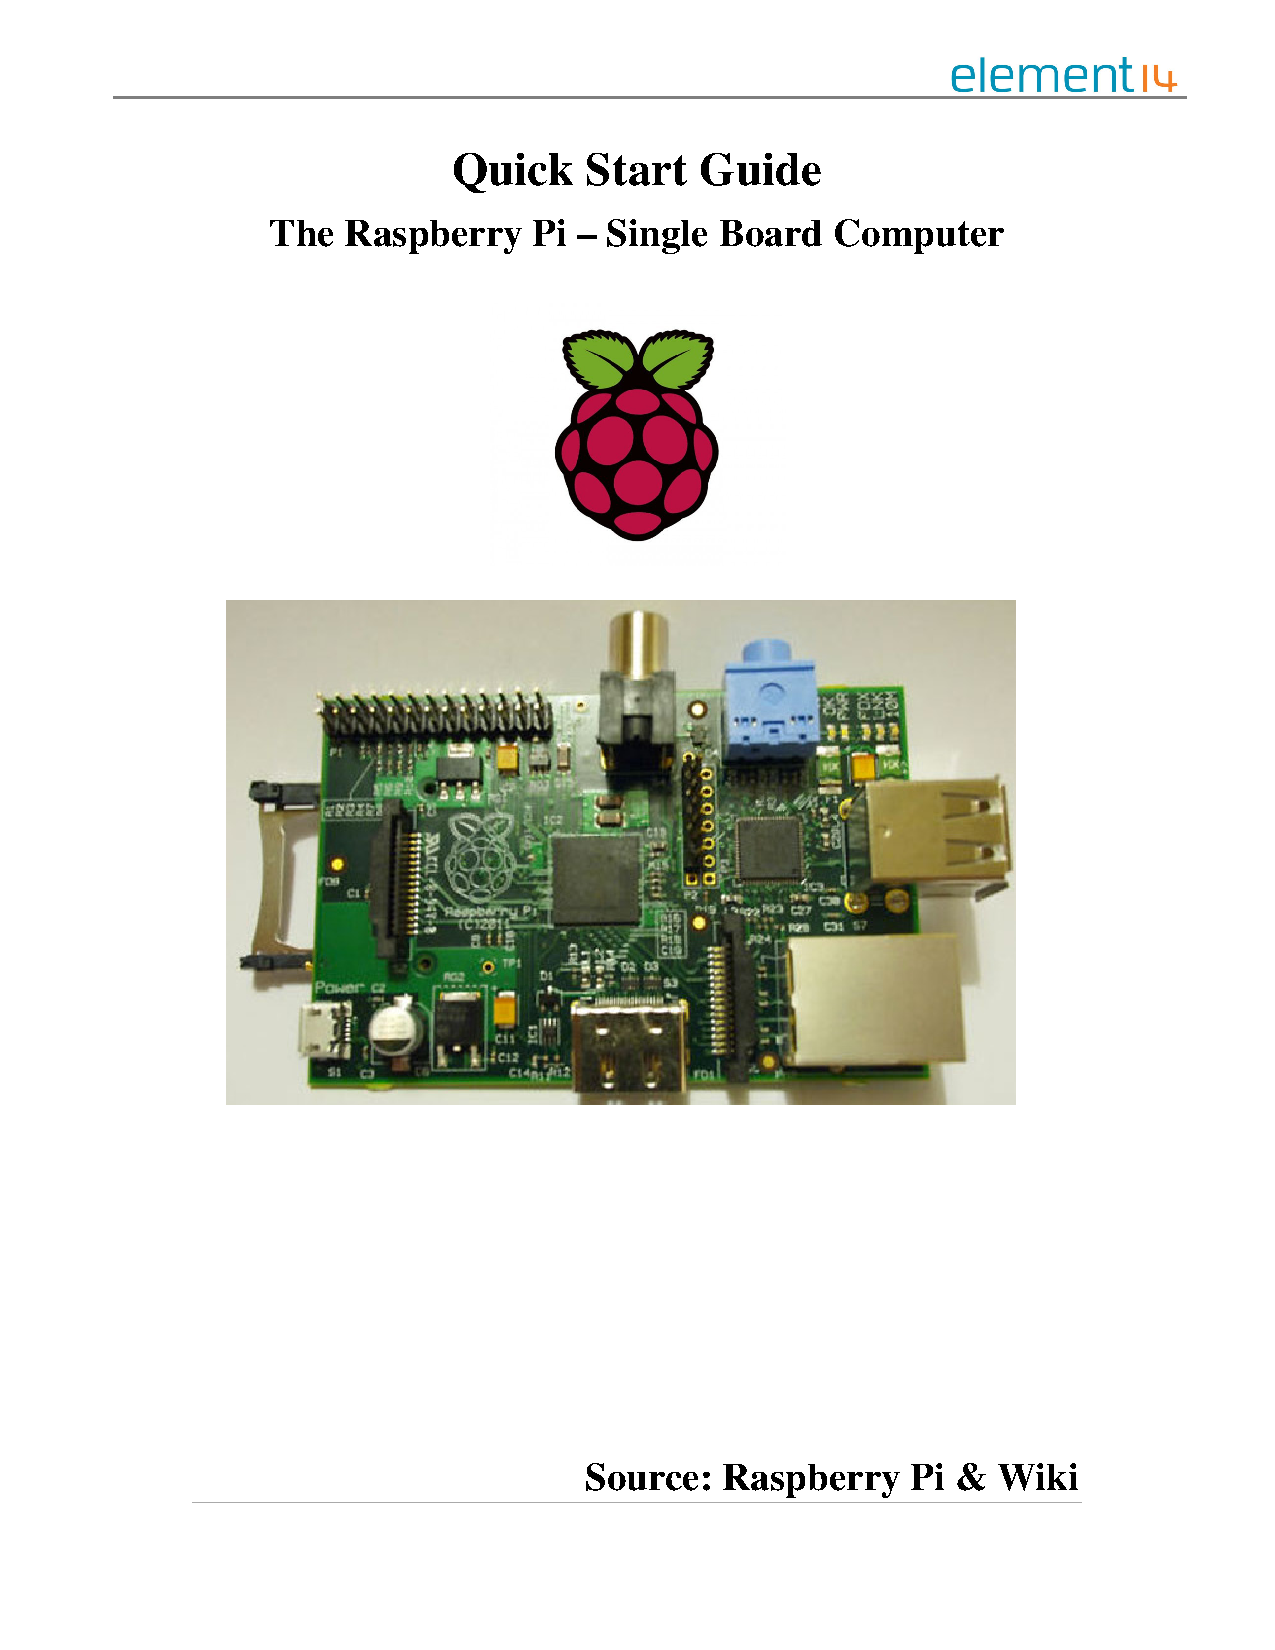
\includepdf[
pages=-,
width=1.6\textwidth,
height=1\textheight,
angle=0,
pagecommand =\section*{Driver Chip}]{datasheets/RaspberryPi_Technical_Data_Sheet.pdf}

\end{document}
